% *******************************************************************
% STOP - Bitte zuerst lesen, bevor Sie weitermachen
%
% Einige Dinge müssen Sie an Ihre Bedürfnisse (und die Vorgaben Ihres
% Betreuers anpassen).
%
% 1. Sprache
% Das Template unterstützt Deutsch und Englisch, Standard ist Deutsch.
% Wenn Sie Englisch verwenden wollen, ändern Sie bitte direkt am Anfang
% dieser Datei den Eintrag
%    \newcommand{\hsmasprache}{de}
% auf
%    \newcommand{\hsmasprache}{en}
%
% 2. Form der Abgabe
% Das Template unterstützt sowohl eine digitale Abgabe, als auch eine Abgabe
% auf Papier. Bei einer Papierabgabe wird ein doppelseitiger Druck vorbereitet
% und der Titel wird so platziert, dass er in das Fenster des offiziellen
% Umschlages der Hochschule passt.
% Bei einer digitalen Abgabe (als PDF) wird der Titel zentriert und als
% Format wird einseitig gewählt. Außerdem wird die Datei unterschrift.png
% auf dem Blatt mit der Erklärung zur Eigenständigkeit eingebunden.
%
% 3. Zitierstil
% Abhängig von dem gewünschten Zitierstil passen Sie bitte in
% preambel.tex die Einstellungen bei \usepackage[backend=biber...
% an. Wie ist dort genau erklärt.
% Achtung: Wenn Sie als Zitierstil Fußnoten wählen bzw. generell
% -------  mit Fußnoten arbeiten, dann beachten Sie bitte, dass
%          Fußnoten in Bildunterschriften und Tabellenüberschriften
%          nicht funktionieren.
%          Siehe hierzu https://texfaq.org/FAQ-ftncapt
%          und https://texfaq.org/FAQ-footintab
%          Sinnvollerweise verzichten Sie auf Fußnoten an diesen
%          Stellen und fügen Quellen einfach per \parancite ein.
%
% 4. Doppelseitiger oder einseitiger Druck
% Das Template bestimmt, ob einseitig oder doppelseitig gedruckt wird
% anhand der Abgabeform (papier / digital). Wollen sie dies übersteuern,
% müssen Sie in der Datei preambel.tex folgende Zeile
% \KOMAoptions{twoside=true} für doppelsetigen Druck
% \KOMAoptions{twoside=false} für einsetigen Druck
% direkt vor \usepackage{xcolor} einsetzen. Prinzipiell sollten Sie aber
% das vorgeschlagene Format einfach so lassen.
%
% 5. Abkürzungen auf richtige Breite einstellen und sortieren
% In der Datei kapitel/abkuerzungen.tex müssen Sie die _längste_
% Abkürzung in die eckigen Klammern von \begin{acronym} schreiben,
% sonst werden die Abkürzungen nicht richtig ausgerichtet.
% Also z.B. \begin{acronym}[DSGVO].
% Außerdem müssen Sie die Abkürzungen selbst (manuell) sortieren,
% da dies nicht automatisch passiert. Am einfachsten verwenden Sie
% hierzu die Sortierfunktion Ihres Texteditors.
%
% 6. Unnötige Teile entfernen
% Entfernen Sie die Teile, die Sie nicht brauchen, z.B. Anhänge,
% Quelltextverzeichnis etc. Siehe unten
%
% 7. Silbentrennung
% LaTeX führt eine automatische Silbentrennung durch. Allerdings
% werden Wörter, die bereits einen Bindestrich enthalten nicht
% getrennt, z.B. Datenschutz-Grundverordnung. Wenn Sie Ihren Text auf
% Deutsch schreiben, können Sie dann alternativ "= für den Bindestrich
% im Wort verwenden, z.B. Datenschutz"=Grundverordnung, damit LaTeX
% weiterhin richtig trennt.
% Ist die Silbentrennung aus einem anderen Grund nicht erfolgt, sodass
% das Wort über den rechten Rand hinaussteht oder wenn Sie eine weitere
% Trennstelle wollen, können Sie LaTeX helfen, indem Sie weitere
% Trennstellen angeben. Dies geschieht durch "- als Zeichen, z.B.
% Staats"-vertrag.
%
% 8. Nummerierung der Fußnoten
% LaTeX beginnt die Nummerierung der Fußnoten in jedem Kapitel wieder
% bei 1. Manche Dozenten wollen aber eine durchlaufende Nummerierung
% über die gesamte Arbeit. In diesem Fall gehen Sie in die preambel.tex
% und kommentieren den Befehl \counterwithout{footnote}{chapter} ein.
%
% 9. Unterschrift
% Bei einer Abgabe auf Papier unterschreiben Sie die Arbeit eigenhändig.
% Geben Sie allerdings digital ab, sollten Sie die Datei unterschrift.png
% durch einen Scan Ihrer eigenen Unteschrift ersetzen - andernfalls
% unterschreiben Sie als Max Mustermann ;-)
% *******************************************************************

% Sprache für das Dokument festlegen
\newcommand{\hsmasprache}{de}     % de oder en für Deutsch oder Englisch

% Abgabeform festlegen
% Bei einer digitalen Abgabe, wird das Dokument einseitig erzeugt und der Titel wird
% zentriert.
\newcommand{\hsmaabgabe}{digital} % Wie erfolgt die Abgabe: "papier" oder "digital"?

% Preambel mit Einstellungen importieren
% Dokumententyp und benutzte Pakete
\documentclass[open=right,  % Kapitel darf nur auf rechten Seite beginnen
    paper=a4,               % DIN-A4-Papier
    fontsize=12pt,          % Schriftgöße
    headings=small,         % Kleine Überschriften
    headsepline=true,       % Trennlinie am Kopf der Seite
    footsepline=false,      % Keine Trennlinie am Fuß der Seite
    bibliography=totoc,     % Literaturverzeichnis in das Inhaltsverzeichnis aufnehmen
    DIV=7,                  % Verhältnis der Ränder zum bedruckten Bereich
    chapterprefix=true,     % Kapitel x vor dem Kapitelnamen
    cleardoublepage=plain]{scrbook}

% Pakete einbinden, die benötigt werden
\usepackage{ifthen}               % Logische Bedingungen mit ifthenelse
\usepackage{scrlayer-scrpage}     % Erweiterte Einstellungen an scrbook zulassen
\usepackage[utf8]{inputenc}       % Dateien in UTF-8 benutzen
\usepackage[T1]{fontenc}          % Zeichenkodierung
\usepackage{graphicx}             % Bilder einbinden
\usepackage{enumitem}             % Eigene Listen definieren können
\usepackage{setspace}             % Abstände korrigieren

% Setzen von Optionen abhängig von der gewählten Sprache. Die Sprache wird
% in thesis.tex gesetzt.
\ifthenelse{\equal{\hsmasprache}{de}}%
  {%
   \usepackage[main=ngerman, english]{babel}              % Deutsche Sprachunterstützung
   \usepackage[autostyle=true,german=quotes]{csquotes}    % Deutsche Anführungszeichen
   \usepackage[pagebackref=false,german]{hyperref}        % Hyperlinks
   \newcommand{\hsmasortlocale}{de_DE}                    % Sortierung der Literatur
  }%
  {%
   \usepackage[main=english, ngerman]{babel}              % Englische Sprachunterstützung
   \usepackage[autostyle=true,english=american]{csquotes} % Englische Anführungszeichen
   \usepackage[pagebackref=false,english]{hyperref}       % Hyperlinks
   \newcommand{\hsmasortlocale}{en_US}                    % Sortierung der Literatur
  }%

% Setzen von Optionen abhängig von der Abgabeform. Die Abgabeform wird
% in thesis.tex gesetzt.
\ifthenelse{\equal{\hsmaabgabe}{papier}}%
  {%
    \KOMAoptions{twoside=true}
    \newcommand{\hsmafenster}{45mm}
  }%
  {%
    \KOMAoptions{twoside=false}
    \newcommand{\hsmafenster}{38.5mm}
  }%

\usepackage{xcolor}               % Unterstützung für Farben
\usepackage{amsmath}              % Mathematische Formeln
\usepackage{amsfonts}             % Mathematische Zeichensätze
\usepackage{amssymb}              % Mathematische Symbole
\usepackage{float}                % Fließende Objekte (Tabellen, Grafiken etc.)
\usepackage{booktabs}             % Korrekter Tabellensatz
\usepackage[printonlyused]{acronym}  % Abkürzungsverzeichnis [nur verwendete Abkürzungen]
\usepackage{makeidx}              % Sachregister
\usepackage{listings}             % Quelltexte
\usepackage{listingsutf8}         % Quelltexte in UTF8
\usepackage[hang,font={sf,footnotesize},labelfont={footnotesize,bf}]{caption} % Beschriftungen
\usepackage[scaled]{helvet}       % Schrift Helvetia laden
\usepackage[absolute]{textpos}    % Absolute Textpositionen (für Deckblatt)
\usepackage{calc}                 % Berechnung von Positionen
\usepackage{blindtext}            % Blindtexte
\usepackage[bottom=40mm,left=35mm,right=35mm,top=30mm]{geometry} % Ränder ändern
\usepackage{scrhack}              % tocbasic Warnung entfernen
\usepackage[all]{hypcap}          % Korrekte Verlinkung von Floats
\usepackage{tabularx}             % Spezielle Tabellen
\usepackage[backend=biber,
  isbn=false,                     % ISBN nicht anzeigen, gleiches geht mit nahezu allen anderen Feldern
  sortlocale=\hsmasortlocale,     % Sortierung der Einträge für Deutsch
                                  %      de_DE: für Deutsch
                                  %      en_US: für Englisch
  autocite=inline,                % regelt Aussehen für \autocite
                                  %      inline: Zitat in Klammern (\parancite)
                                  %      footnote: Zitat in Fußnoten (\footcite)
                                  %      plain: Zitat direkt ohne Klammern (\cite)
  style=ieee,                     % Legt den Stil für die Zitate fest
                                  %      ieee: Zitate als Zahlen [1]
                                  %      alphabetic: Zitate als Kürzel und Jahr [Ein05]
                                  %      authoryear: Zitate Author und Jahr [Einstein (1905)]
  hyperref=true,                  % Hyperlinks für Zitate
  firstinits=false                % Vornamen abkürzen (Maier, M. anstatt Maier, Markus)?
                                  %      true: abkürzen
                                  %      false: nicht abkürzen
]{biblatex}                       % Literaturverwaltung mit BibLaTeX
\usepackage{rotating}             % Seiten drehen
\usepackage{harveyballs}          % Harveyballs
\usepackage{chngcntr}             % Counter (Zähler) ändern können - für Fußnotennummern
\usepackage{longtable}            % Tabellen, die mehr als eine Seite umfassen
\usepackage{tikz}                 % tikz für graphiken (neuronale netze oder schachfelder)

% Einstellungen zu den Fußnoten
\renewcommand{\footnotesize}{\fontsize{9}{10}\selectfont} % Größe der Fußnoten
\setlength{\footnotesep}{8pt} % Abstand zwischen den Fußnoten

% Kommentieren Sie diese Zeile ein, wenn Sie eine "durchlaufende" Nummerierung bei den
% Fußnoten wünschen, d.h. wenn die Fußnoten nicht bei jedem Kapitel wieder bei 1
% beginnen sollen.
%\counterwithout{footnote}{chapter}

\setlength{\bibitemsep}{1em}      % Abstand zwischen den Literaturangaben
\setlength{\bibhang}{2em}         % Einzug nach jeweils erster Zeile

% Trennung von URLs im Literaturverzeichnis (große Werte [> 10000] verhindern die Trennung)
\defcounter{biburlnumpenalty}{10} % Strafe für Trennung in URL nach Zahl
\defcounter{biburlucpenalty}{500} % Strafe für Trennung in URL nach Großbuchstaben
\defcounter{biburllcpenalty}{500} % Strafe für Trennung in URL nach Kleinbuchstaben

% Farben definieren
\definecolor{linkblue}{RGB}{0, 0, 100}
\definecolor{linkblack}{RGB}{0, 0, 0}
\definecolor{comment}{RGB}{63, 127, 95}
\definecolor{darkgreen}{RGB}{14, 144, 102}
\definecolor{darkblue}{RGB}{0,0,168}
\definecolor{darkred}{RGB}{128,0,0}
\definecolor{javadoccomment}{RGB}{0,0,240}

% Einstellungen für das Hyperlink-Paket
\hypersetup{
    colorlinks=true,      % Farbige links verwenden
%    allcolors=linkblue,
    linktoc=all,          % Links im Inhaltsverzeichnis
    linkcolor=linkblack,  % Querverweise
    citecolor=linkblack,  % Literaturangaben
    filecolor=linkblack,  % Dateilinks
    urlcolor=linkblack    % URLs
}

% Einstellungen für Quelltexte
\lstset{
      xleftmargin=0.2cm,
      basicstyle=\footnotesize\ttfamily,
      keywordstyle=\color{darkgreen},
      identifierstyle=\color{darkblue},
      commentstyle=\color{comment},
      stringstyle=\color{darkred},
      tabsize=2,
      lineskip={2pt},
      columns=flexible,
      inputencoding=utf8,
      captionpos=b,
      breakautoindent=true,
      breakindent=2em,
      breaklines=true,
      prebreak=,
      postbreak=,
      numbers=none,
      numberstyle=\tiny,
      showspaces=false,      % Keine Leerzeichensymbole
      showtabs=false,        % Keine Tabsymbole
      showstringspaces=false,% Leerzeichen in Strings
      morecomment=[s][\color{javadoccomment}]{/**}{*/},
      literate={Ö}{{\"O}}1 {Ä}{{\"A}}1 {Ü}{{\"U}}1 {ß}{{\ss}}2 {ü}{{\"u}}1 {ä}{{\"a}}1 {ö}{{\"o}}1
}

\urlstyle{same}

% Einstellungen für Überschriften
\renewcommand*{\chapterformat}{%
  \Large\chapapp~\thechapter   % Große Schrift
  \vspace{0.3cm}               % Abstand zum Titel des Kapitels
}

% Abstände für die Überschriften setzen
\renewcommand{\chapterheadstartvskip}{\vspace*{2.6cm}}
\renewcommand{\chapterheadendvskip}{\vspace*{1.5cm}}

% Vertikale Abstände für die Überschriften etwas verkleinern
\RedeclareSectionCommand[
  beforeskip=-1.8\baselineskip,
  afterskip=0.25\baselineskip]{section}

\RedeclareSectionCommand[
  beforeskip=-1.8\baselineskip,
  afterskip=0.15\baselineskip]{subsection}

\RedeclareSectionCommand[
  beforeskip=-1.8\baselineskip,
  afterskip=0.15\baselineskip]{subsubsection}

% In der Kopfzeile nur die kurze Kapitelbezeichnung (ohne Kapitel davor)
\renewcommand*\chaptermarkformat{\thechapter\autodot\enskip}
\automark[chapter]{chapter}

% Einstellungen für Schriftarten
\setkomafont{pagehead}{\normalfont\sffamily}
\setkomafont{pagenumber}{\normalfont\sffamily}
\setkomafont{paragraph}{\sffamily\bfseries\small}
\setkomafont{subsubsection}{\sffamily\itshape\bfseries\small}
\addtokomafont{footnote}{\footnotesize}
\setkomafont{chapter}{\LARGE\selectfont\bfseries}

% Wichtige Abstände
\setlength{\parskip}{0.2cm}  % 2mm Abstand zwischen zwei Absätzen
\setlength{\parindent}{0mm}  % Absätze nicht einziehen
\clubpenalty = 10000         % Keine "Schusterjungen"
\widowpenalty = 10000        % Keine "Hurenkinder"
\displaywidowpenalty = 10000 % Keine "Hurenkinder"
                             % Siehe: https://de.wikipedia.org/wiki/Hurenkind_und_Schusterjunge

% Index erzeugen
\makeindex

% Einfacher Font-Wechsel über dieses Makro
\newcommand{\changefont}[3]{
\fontfamily{#1} \fontseries{#2} \fontshape{#3} \selectfont}

% Eigenes Makro für Bilder. Das label (für \ref) ist dann einfach
% der Name der Bilddatei
\newcommand{\bild}[3]{
\begin{figure}[ht]
  \centering
  \includegraphics[width=#2]{#1}
  \caption{#3}
  \label{#1}
\end{figure}}

% Wo liegt Sourcecode?
\newcommand{\srcloc}{src/}

% Wo sind die Bilder?
\graphicspath{{bilder/}}

% Makros für typographisch korrekte Abkürzungen
\newcommand{\zb}[0]{z.\,B.}
\newcommand{\dahe}[0]{d.\,h.}
\newcommand{\ua}[0]{u.\,a.}

% Flags für Veröffentlichung und Sperrvermerk
\newboolean{hsmapublizieren}
\newboolean{hsmasperrvermerk}

% Tabellenzellen mit mehreren Zeilen
\newcolumntype{L}{>{\raggedright\arraybackslash}X}
\newcolumntype{b}{l}
\newcolumntype{s}{>{\hsize=.3\hsize}l}
\newcolumntype{F}{>{\hsize=\dimexpr2\hsize+2\tabcolsep+\arrayrulewidth\relax}X}

% Checklisten mit zwei Ebenen
\newlist{checklist}{itemize}{2}
\setlist[checklist]{label=$\square$}

% tikz setup
\usetikzlibrary{positioning}

% Dokumenteninfos importieren
% -------------------------------------------------------
% Daten für die Arbeit
% Wenn hier alles korrekt eingetragen wurde, wird das Titelblatt
% automatisch generiert. D.h. die Datei titelblatt.tex muss nicht mehr
% angepasst werden.

% Titel der Arbeit auf Deutsch
\newcommand{\hsmatitelde}{Entwicklung eines \ac{NNUE} zur Evaluation von Schachpositionen}

% Titel der Arbeit auf Englisch
\newcommand{\hsmatitelen}{Development of an \ac{NNUE} for the Evaluation of Chess Positions}

% Weitere Informationen zur Arbeit
\newcommand{\hsmaort}{Mannheim}          % Ort
\newcommand{\hsmaautorvname}{Marvin}        % Vorname(n)
\newcommand{\hsmaautornname}{Karhan} % Nachname(n)
\newcommand{\hsmadatum}{28.09.2022}      % Datum der Abgabe
\newcommand{\hsmajahr}{2022}             % Jahr der Abgabe
\newcommand{\hsmafirma}{} % Firma bei der die Arbeit durchgeführt wurde
\newcommand{\hsmabetreuer}{Prof. Dr. Jörn Fischer, Hochschule Mannheim} % Betreuer an der Hochschule
\newcommand{\hsmazweitkorrektor}{Prof. Dr. Thomas Ihme, Hochschule Mannheim}   % Betreuer im Unternehmen oder Zweitkorrektor
\newcommand{\hsmafakultaet}{I}    % I für Informatik oder E, S, B, D, M, N, W, V
\newcommand{\hsmastudiengang}{IB} % IB IMB UIB CSB IM MTB (weitere siehe titleblatt.tex)

% Zustimmung zur Veröffentlichung
\setboolean{hsmapublizieren}{true}   % Einer Veröffentlichung wird zugestimmt
\setboolean{hsmasperrvermerk}{false} % Die Arbeit hat keinen Sperrvermerk

% -------------------------------------------------------
% Abstract
% Achtung: Wenn Sie im Abstrakt Anführungszeichen verwenden wollen, dann benutzen Sie
%          nicht "` und "', sondern \enquote{}. "` und "' werden nicht richtig
%          erkannt.

% Kurze (maximal halbseitige) Beschreibung, worum es in der Arbeit geht auf Deutsch
\newcommand{\hsmaabstractde}{Abstract}

% Kurze (maximal halbseitige) Beschreibung, worum es in der Arbeit geht auf Englisch
\newcommand{\hsmaabstracten}{Abstract}


% Richtige Titel für das Quellcodeverzeichnis
\renewcommand\lstlistingname{\hsmalistings}
\renewcommand\lstlistlistingname{\hsmalistings}

% Literatur-Datenbank
\addbibresource{literatur.bib}   % BibLaTeX-Datei mit Literaturquellen einbinden

% Anfang des Dokuments
\begin{document}
\frontmatter

% Römische Ziffern für die "Front-Matter"
\setcounter{page}{0}
\changefont{ptm}{m}{n}  % Times New Roman für den Fließtext
\renewcommand{\rmdefault}{ptm}

% Titelblatt
% *******************************************************************
% In dieser Datei sollten eigentlich keine Veränderungen
% notwendig sein. Alle Einstellungen erfolgen in docinfo.tex und
% der thesis.tex.
% *******************************************************************

\thispagestyle{empty}

% Fakultäten der HS-Mannheim
% *******************************************************************
\ifthenelse{\equal{\hsmafakultaet}{I}}%
  {\newcommand{\hsmafakultaetlangde}{Fakultät für Informatik}%
   \newcommand{\hsmafakultaetlangen}{Department of Computer Science}}{}

\ifthenelse{\equal{\hsmafakultaet}{E}}%
  {\newcommand{\hsmafakultaetlangde}{Fakultät für Elektrotechnik}%
   \newcommand{\hsmafakultaetlangen}{Department of Electrical Engineering}}{}

\ifthenelse{\equal{\hsmafakultaet}{S}}%
  {\newcommand{\hsmafakultaetlangde}{Fakultät für Sozialwesen}%
   \newcommand{\hsmafakultaetlangen}{Department of Social Work}}{}

\ifthenelse{\equal{\hsmafakultaet}{B}}%
  {\newcommand{\hsmafakultaetlangde}{Fakultät für Biotechnologie}%
   \newcommand{\hsmafakultaetlangen}{Department of Biotechnology}}{}

\ifthenelse{\equal{\hsmafakultaet}{D}}%
  {\newcommand{\hsmafakultaetlangde}{Fakultät für Gestaltung}%
   \newcommand{\hsmafakultaetlangen}{Department of Design}}{}

\ifthenelse{\equal{\hsmafakultaet}{M}}%
  {\newcommand{\hsmafakultaetlangde}{Fakultät für Maschinenbau}%
   \newcommand{\hsmafakultaetlangen}{Department of Mechanical Engineering}}{}

\ifthenelse{\equal{\hsmafakultaet}{N}}%
  {\newcommand{\hsmafakultaetlangde}{Fakultät für Informationstechnik}%
   \newcommand{\hsmafakultaetlangen}{Department of Information Technology}}{}

\ifthenelse{\equal{\hsmafakultaet}{W}}%
  {\newcommand{\hsmafakultaetlangde}{Fakultät für Wirtschaftsingenieurwesen}%
   \newcommand{\hsmafakultaetlangen}{Department of Engineering and Management}}{}

\ifthenelse{\equal{\hsmafakultaet}{V}}%
  {\newcommand{\hsmafakultaetlangde}{Fakultät für Verfahrens- und Chemietechnik}%
   \newcommand{\hsmafakultaetlangen}{Department of Chemical Process Engineering}}{}

% Studiengänge der HS-Mannheim
% *******************************************************************
\ifthenelse{\equal{\hsmastudiengang}{IB}}%
  {\newcommand{\hsmastudienganglangde}{Informatik}%
  \newcommand{\hsmastudienganglangen}{Computer Science}%
  \newcommand{\hsmatypde}{Bachelor-Thesis}%
  \newcommand{\hsmatypen}{Bachelor Thesis}%
  \newcommand{\hsmagrad}{\hsmabsc}}{}

\ifthenelse{\equal{\hsmastudiengang}{IMB}}%
  {\newcommand{\hsmastudienganglangde}{Medizinische Informatik}%
  \newcommand{\hsmastudienganglangen}{Medical Informatics}%
  \newcommand{\hsmatypde}{Bachelor-Thesis}%
  \newcommand{\hsmatypen}{Bachelor Thesis}%
  \newcommand{\hsmagrad}{\hsmabsc}}{}

\ifthenelse{\equal{\hsmastudiengang}{UIB}}%
  {\newcommand{\hsmastudienganglangde}{Unternehmens- und Wirtschaftsinformatik}%
  \newcommand{\hsmastudienganglangen}{Enterprise Computing}%
  \newcommand{\hsmatypde}{Bachelor-Thesis}%
  \newcommand{\hsmatypen}{Bachelor Thesis}%
  \newcommand{\hsmagrad}{\hsmabsc}}{}

\ifthenelse{\equal{\hsmastudiengang}{CSB}}%
  {\newcommand{\hsmastudienganglangde}{Cyber Security}%
  \newcommand{\hsmastudienganglangen}{Cyber Security}%
  \newcommand{\hsmatypde}{Bachelor-Thesis}%
  \newcommand{\hsmatypen}{Bachelor Thesis}%
  \newcommand{\hsmagrad}{\hsmabsc}}{}

\ifthenelse{\equal{\hsmastudiengang}{IM}}%
  {\newcommand{\hsmastudienganglangde}{Informatik}%
   \newcommand{\hsmastudienganglangen}{Computer Science}%
   \newcommand{\hsmatypde}{Master-Thesis}%
   \newcommand{\hsmatypen}{Master Thesis}%
   \newcommand{\hsmagrad}{\hsmamaster}}{}

\ifthenelse{\equal{\hsmastudiengang}{MEB}}%
  {\newcommand{\hsmastudienganglangde}{Mechatronik}%
   \newcommand{\hsmastudienganglangen}{Mechatronic}%
   \newcommand{\hsmatypde}{Bachelor-Thesis}%
   \newcommand{\hsmatypen}{Bachelor Thesis}%
   \newcommand{\hsmagrad}{\hsmabsc}}{}

\ifthenelse{\equal{\hsmastudiengang}{UB}}%
  {\newcommand{\hsmastudienganglangde}{Automatisierungstechnik}%
   \newcommand{\hsmastudienganglangen}{Automation Technology}%
   \newcommand{\hsmatypde}{Bachelor-Thesis}%
   \newcommand{\hsmatypen}{Bachelor Thesis}%
   \newcommand{\hsmagrad}{\hsmabsc}}{}

\ifthenelse{\equal{\hsmastudiengang}{ELB}}%
  {\newcommand{\hsmastudienganglangde}{Elektro- und Informationstechnik/Ingenieurpädagogik}%
   \newcommand{\hsmastudienganglangen}{Elektro- und Informationstechnik/Ingenieurpädagogik}%
   \newcommand{\hsmatypde}{Bachelor-Thesis}%
   \newcommand{\hsmatypen}{Bachelor Thesis}%
   \newcommand{\hsmagrad}{\hsmabsc}}{}

\ifthenelse{\equal{\hsmastudiengang}{EBE}}%
  {\newcommand{\hsmastudienganglangde}{Energietechnik und erneuerbare Energien}%
   \newcommand{\hsmastudienganglangen}{Power Engineering ans Renewable Energies}%
   \newcommand{\hsmatypde}{Bachelor-Thesis}%
   \newcommand{\hsmatypen}{Bachelor Thesis}%
   \newcommand{\hsmagrad}{\hsmabsc}}{}

\ifthenelse{\equal{\hsmastudiengang}{TS}}%
  {\newcommand{\hsmastudienganglangde}{Translation Studies}%
   \newcommand{\hsmastudienganglangen}{Translation Studies}%
   \newcommand{\hsmatypde}{Bachelor-Thesis}%
   \newcommand{\hsmatypen}{Bachelor Thesis}%
   \newcommand{\hsmagrad}{\hsmabsc}}{}

\ifthenelse{\equal{\hsmastudiengang}{EM}}%
  {\newcommand{\hsmastudienganglangde}{Automatisierungs- und Energiesysteme}%
   \newcommand{\hsmastudienganglangen}{Automation and Energy Systems}%
   \newcommand{\hsmatypde}{Master-Thesis}%
   \newcommand{\hsmatypen}{Master Thesis}%
   \newcommand{\hsmagrad}{\hsmamaster}}{}

\ifthenelse{\equal{\hsmastudiengang}{ELM}}%
  {\newcommand{\hsmastudienganglangde}{Lehramt Ingenieurpädagogik}%
   \newcommand{\hsmastudienganglangen}{Lectureship Educational Engineering}%
   \newcommand{\hsmatypde}{Master-Thesis}%
   \newcommand{\hsmatypen}{Master Thesis}%
   \newcommand{\hsmagrad}{\hsmamaster}}{}

\ifthenelse{\equal{\hsmastudiengang}{SAB}}%
  {\newcommand{\hsmastudienganglangde}{Soziale Arbeit}%
   \newcommand{\hsmastudienganglangen}{Social Labour}%
   \newcommand{\hsmatypde}{Bachelor-Thesis}%
   \newcommand{\hsmatypen}{Bachelor Thesis}%
   \newcommand{\hsmagrad}{\hsmaba}}{}

\ifthenelse{\equal{\hsmastudiengang}{SAM}}%
  {\newcommand{\hsmastudienganglangde}{Soziale Arbeit}%
   \newcommand{\hsmastudienganglangen}{Social Labour}%
   \newcommand{\hsmatypde}{Master-Thesis}%
   \newcommand{\hsmatypen}{Master Thesis}%
   \newcommand{\hsmagrad}{\hsmamastera}}{}

\ifthenelse{\equal{\hsmastudiengang}{BB}}%
  {\newcommand{\hsmastudienganglangde}{Biotechnology}%
   \newcommand{\hsmastudienganglangen}{Biotechnology}%
   \newcommand{\hsmatypde}{Bachelor-Thesis}%
   \newcommand{\hsmatypen}{Bachelor Thesis}%
   \newcommand{\hsmagrad}{\hsmabsc}}{}

\ifthenelse{\equal{\hsmastudiengang}{BCB}}%
  {\newcommand{\hsmastudienganglangde}{Biologische Chemie}%
   \newcommand{\hsmastudienganglangen}{Biological Chemics}%
   \newcommand{\hsmatypde}{Bachelor-Thesis}%
   \newcommand{\hsmatypen}{Bachelor Thesis}%
   \newcommand{\hsmagrad}{\hsmabsc}}{}

\ifthenelse{\equal{\hsmastudiengang}{BMEBST}}%
  {\newcommand{\hsmastudienganglangde}{Biotechnology - Biomedical Science and Technology}%
   \newcommand{\hsmastudienganglangen}{Biotechnology - Biomedical Science and Technology}%
   \newcommand{\hsmatypde}{Master-Thesis}%
   \newcommand{\hsmatypen}{Master Thesis}%
   \newcommand{\hsmagrad}{\hsmamaster}}{}

\ifthenelse{\equal{\hsmastudiengang}{BMEBPD}}%
  {\newcommand{\hsmastudienganglangde}{Biotechnology - Bioprocess Development}%
   \newcommand{\hsmastudienganglangen}{Biotechnology - Bioprocess Development}%
   \newcommand{\hsmatypde}{Master-Thesis}%
   \newcommand{\hsmatypen}{Master Thesis}%
   \newcommand{\hsmagrad}{\hsmamaster}}{}

\ifthenelse{\equal{\hsmastudiengang}{BLSM}}%
  {\newcommand{\hsmastudienganglangde}{Life Science Management}%
   \newcommand{\hsmastudienganglangen}{Life Science Management}%
   \newcommand{\hsmatypde}{Master-Thesis}%
   \newcommand{\hsmatypen}{Master Thesis}%
   \newcommand{\hsmagrad}{\hsmamaster}}{}

\ifthenelse{\equal{\hsmastudiengang}{KDB}}%
  {\newcommand{\hsmastudienganglangde}{Kommunikationsdesign}%
   \newcommand{\hsmastudienganglangen}{Communication Design}%
   \newcommand{\hsmatypde}{Bachelor-Thesis}%
   \newcommand{\hsmatypen}{Bachelor Thesis}%
   \newcommand{\hsmagrad}{\hsmaba}}{}

\ifthenelse{\equal{\hsmastudiengang}{KDM}}%
  {\newcommand{\hsmastudienganglangde}{Kommunikationsdesign}%
   \newcommand{\hsmastudienganglangen}{Communication Design}%
   \newcommand{\hsmatypde}{Master-Thesis}%
   \newcommand{\hsmatypen}{Master Thesis}%
   \newcommand{\hsmagrad}{\hsmamastera}}{}

\ifthenelse{\equal{\hsmastudiengang}{MB}}%
  {\newcommand{\hsmastudienganglangde}{Maschinenbau}%
   \newcommand{\hsmastudienganglangen}{Mechanical Engineering}%
   \newcommand{\hsmatypde}{Bachelor-Thesis}%
   \newcommand{\hsmatypen}{Bachelor Thesis}%
   \newcommand{\hsmagrad}{\hsmabsc}}{}

\ifthenelse{\equal{\hsmastudiengang}{MM}}%
  {\newcommand{\hsmastudienganglangde}{Maschinenbau}%
   \newcommand{\hsmastudienganglangen}{Mechanical Engineering}%
   \newcommand{\hsmatypde}{Master-Thesis}%
   \newcommand{\hsmatypen}{Master Thesis}%
   \newcommand{\hsmagrad}{\hsmamaster}}{}

\ifthenelse{\equal{\hsmastudiengang}{NEB}}%
  {\newcommand{\hsmastudienganglangde}{Elektronik}%
   \newcommand{\hsmastudienganglangen}{Electronics}%
   \newcommand{\hsmatypde}{Bachelor-Thesis}%
   \newcommand{\hsmatypen}{Bachelor Thesis}%
   \newcommand{\hsmagrad}{\hsmabsc}}{}

\ifthenelse{\equal{\hsmastudiengang}{TIB}}%
  {\newcommand{\hsmastudienganglangde}{Technische Informatik}%
   \newcommand{\hsmastudienganglangen}{Technical Information Technology}%
   \newcommand{\hsmatypde}{Bachelor-Thesis}%
   \newcommand{\hsmatypen}{Bachelor Thesis}%
   \newcommand{\hsmagrad}{\hsmabsc}}{}

\ifthenelse{\equal{\hsmastudiengang}{MTB}}%
  {\newcommand{\hsmastudienganglangde}{Medizintechnik}%
   \newcommand{\hsmastudienganglangen}{Medical Technology}%
   \newcommand{\hsmatypde}{Bachelor-Thesis}%
   \newcommand{\hsmatypen}{Bachelor Thesis}%
   \newcommand{\hsmagrad}{\hsmabsc}}{}

\ifthenelse{\equal{\hsmastudiengang}{MTM}}%
  {\newcommand{\hsmastudienganglangde}{Medizintechnik}%
   \newcommand{\hsmastudienganglangen}{Medical Technology}%
   \newcommand{\hsmatypde}{Master-Thesis}%
   \newcommand{\hsmatypen}{Master Thesis}%
   \newcommand{\hsmagrad}{\hsmamaster}}{}

\ifthenelse{\equal{\hsmastudiengang}{NM}}%
  {\newcommand{\hsmastudienganglangde}{Informationstechnik}%
   \newcommand{\hsmastudienganglangen}{Informationstechnik}%
   \newcommand{\hsmatypde}{Master-Thesis}%
   \newcommand{\hsmatypen}{Master Thesis}%
   \newcommand{\hsmagrad}{\hsmamaster}}{}

\ifthenelse{\equal{\hsmastudiengang}{WB}}%
  {\newcommand{\hsmastudienganglangde}{Wirtschaftsingenieurwesen}%
   \newcommand{\hsmastudienganglangen}{Engineering and Management}%
   \newcommand{\hsmatypde}{Bachelor-Thesis}%
   \newcommand{\hsmatypen}{Bachelor Thesis}%
   \newcommand{\hsmagrad}{\hsmabsc}}{}

\ifthenelse{\equal{\hsmastudiengang}{WM}}%
  {\newcommand{\hsmastudienganglangde}{Wirtschaftsingenieurwesen}%
   \newcommand{\hsmastudienganglangen}{Engineering and Management}%
   \newcommand{\hsmatypde}{Master-Thesis}%
   \newcommand{\hsmatypen}{Master Thesis}%
   \newcommand{\hsmagrad}{\hsmamaster}}{}

\ifthenelse{\equal{\hsmastudiengang}{WMI}}%
  {\newcommand{\hsmastudienganglangde}{Wirtschaftsingenieurwesen}%
   \newcommand{\hsmastudienganglangen}{Engineering and Management}%
   \newcommand{\hsmatypde}{Master-Thesis}%
   \newcommand{\hsmatypen}{Master Thesis}%
   \newcommand{\hsmagrad}{\hsmamaster}}{}

\ifthenelse{\equal{\hsmastudiengang}{WMB}}%
  {\newcommand{\hsmastudienganglangde}{Wirtschaftsingenieurwesen mit den\\ ingenieurwissenschaftlichen Fachrichtungen Maschinenbau und Elektrotechnik}%
   \newcommand{\hsmastudienganglangen}{Engineering and Management\\ with focus on Mechanical and Electrical Engineering}%
   \newcommand{\hsmatypde}{Master-Thesis}%
   \newcommand{\hsmatypen}{Master Thesis}%
   \newcommand{\hsmagrad}{\hsmamaster}}{}

\ifthenelse{\equal{\hsmastudiengang}{WMW}}%
  {\newcommand{\hsmastudienganglangde}{Wirtschaftsingenieurwesen mit\\ ingenieurwissenschaftlicher Vertiefung des Maschinenbaus}%
   \newcommand{\hsmastudienganglangen}{Engineering and Management\\ deepening the engineering aspects of Mechanical Engineering}%
   \newcommand{\hsmatypde}{Master-Thesis}%
   \newcommand{\hsmatypen}{Master Thesis}%
   \newcommand{\hsmagrad}{\hsmamaster}}{}

\ifthenelse{\equal{\hsmastudiengang}{VB}}%
  {\newcommand{\hsmastudienganglangde}{Verfahrenstechnik}%
   \newcommand{\hsmastudienganglangen}{Process Engineering}%
   \newcommand{\hsmatypde}{Bachelor-Thesis}%
   \newcommand{\hsmatypen}{Bachelor Thesis}%
   \newcommand{\hsmagrad}{\hsmabsc}}{}

\ifthenelse{\equal{\hsmastudiengang}{CB}}%
  {\newcommand{\hsmastudienganglangde}{Chemische Technik}%
   \newcommand{\hsmastudienganglangen}{Chemical Engineering}%
   \newcommand{\hsmatypde}{Bachelor-Thesis}%
   \newcommand{\hsmatypen}{Bachelor Thesis}%
   \newcommand{\hsmagrad}{\hsmabsc}}{}

\ifthenelse{\equal{\hsmastudiengang}{CM}}%
  {\newcommand{\hsmastudienganglangde}{Chemieingenieurwesen}%
   \newcommand{\hsmastudienganglangen}{Chemical Engineering}%
   \newcommand{\hsmatypde}{Master-Thesis}%
   \newcommand{\hsmatypen}{Master Thesis}%
   \newcommand{\hsmagrad}{\hsmamaster}}{}

% Abschlüsse
% *******************************************************************
\newcommand{\hsmabsc}{Bachelor of Science (B.Sc.)}
\newcommand{\hsmaba}{Bachelor of Arts (B.A.)}
\newcommand{\hsmamaster}{Master of Science (M.Sc.)}
\newcommand{\hsmamastera}{Master of Arts (M.A.)}
\newcommand{\hsmamasterba}{Master of Business Administration (MBA)}

\newcommand{\hsmakoerperschaftde}{Hochschule Mannheim}
\newcommand{\hsmakoerperschaften}{University of Applied Sciences Mannheim}

\newcommand{\hsmaautorbib}{\hsmaautornname, \hsmaautorvname} % Autor Nachname, Vorname
\newcommand{\hsmaautor}{\hsmaautorvname \ \hsmaautornname} % Autor Vorname Nachname

\ifthenelse{\equal{\hsmasprache}{de}}%
  {\newcommand{\hsmatyp}{\hsmatypde}%
   \newcommand{\hsmathesistype}{zur Erlangung des akademischen Grades \hsmagrad}%
   \newcommand{\hsmakoerperschaft}{\hsmakoerperschaftde}%
   \newcommand{\hsmastudiengangname}{Studiengang \hsmastudienganglangde}%
   \newcommand{\hsmastudienganglang}{\hsmastudienganglangde}%
   \newcommand{\hsmatitel}{\hsmatitelde}%
   \newcommand{\hsmatutor}{Betreuer}%
   \newcommand{\hsmafakultaetlang}{\hsmafakultaetlangde}%
   \newcommand{\hsmalistoftables}{Tabellenverzeichnis}%
   \newcommand{\hsmalistoffigures}{Abbildungsverzeichnis}%
   \newcommand{\hsmalistings}{Quellcodeverzeichnis}%
   \newcommand{\hsmaindex}{Index}%
   \newcommand{\hsmaabbreviations}{Abkürzungsverzeichnis}%
   \newcommand{\hsmasnowcardanforderung}{Anforderung}%
   \newcommand{\hsmasnowcardno}{Nr}%
   \newcommand{\hsmasnowcardart}{Art}%
   \newcommand{\hsmasnowcardprio}{Prio}%
   \newcommand{\hsmasnowcardtitel}{Titel}%
   \newcommand{\hsmasnowcardherkunft}{Herkunft}%
   \newcommand{\hsmasnowcardkonflikt}{Konflikte}%
   \newcommand{\hsmasnowcardbeschreibung}{Beschreibung}%
   \newcommand{\hsmasnowcardfitkriterium}{Fit-Kriterium}%
   \newcommand{\hsmasnowcardmaterial}{Weiteres Material}%
   \newcommand{\hsmaqasanforderung}{QAS}%
   \newcommand{\hsmaqasno}{Nr}%
   \newcommand{\hsmaqasart}{Art}%
   \newcommand{\hsmaqasprio}{Prio}%
   \newcommand{\hsmaqastitel}{Titel}%
   \newcommand{\hsmaqasquelle}{Quelle}%
   \newcommand{\hsmaqasstimulus}{Stimulus}%
   \newcommand{\hsmaqasartefakt}{Artefakt}%
   \newcommand{\hsmaqasumgebung}{Umgebung}%
   \newcommand{\hsmaqasantwort}{Antwort}%
   \newcommand{\hsmaqasmass}{Maß für Antwort}%
   \selectlanguage{ngerman}}%
  {\newcommand{\hsmatyp}{\hsmatypen}%
   \newcommand{\hsmathesistype}{for the acquisition of the academic degree \hsmagrad}%
   \newcommand{\hsmakoerperschaft}{\hsmakoerperschaften}%
   \newcommand{\hsmastudiengangname}{Course of Studies: \hsmastudienganglang}%
   \newcommand{\hsmastudienganglang}{\hsmastudienganglangen}%
   \newcommand{\hsmatitel}{\hsmatitelen}%
   \newcommand{\hsmatutor}{Tutors}
   \newcommand{\hsmafakultaetlang}{\hsmafakultaetlangen}%
   \newcommand{\hsmalistoftables}{List of Tables}%
   \newcommand{\hsmalistoffigures}{List of Figures}%
   \newcommand{\hsmalistings}{Listings}%
   \newcommand{\hsmaindex}{Index}%
   \newcommand{\hsmaabbreviations}{List of Abbreviations}%
   \newcommand{\hsmasnowcardanforderung}{Requirement}%
   \newcommand{\hsmasnowcardno}{\#}%
   \newcommand{\hsmasnowcardart}{Type}%
   \newcommand{\hsmasnowcardprio}{Prio}%
   \newcommand{\hsmasnowcardtitel}{Title}%
   \newcommand{\hsmasnowcardherkunft}{Origin}%
   \newcommand{\hsmasnowcardkonflikt}{Conflicts}%
   \newcommand{\hsmasnowcardbeschreibung}{Description}%
   \newcommand{\hsmasnowcardfitkriterium}{Fit Criterion}%
   \newcommand{\hsmasnowcardmaterial}{Supporting Material}%
   \newcommand{\hsmaqasanforderung}{QAS}%
   \newcommand{\hsmaqasno}{\#}%
   \newcommand{\hsmaqasart}{Type}%
   \newcommand{\hsmaqasprio}{Prio}%
   \newcommand{\hsmaqastitel}{Title}%
   \newcommand{\hsmaqasquelle}{Source}%
   \newcommand{\hsmaqasstimulus}{Stimulus}%
   \newcommand{\hsmaqasartefakt}{Artifact}%
   \newcommand{\hsmaqasumgebung}{Environment}%
   \newcommand{\hsmaqasantwort}{Response}%
   \newcommand{\hsmaqasmass}{Response Measure}%
   \selectlanguage{english}}%

% Daten in die Standard-Felder von KOMA-Script eintragen
\titlehead{\hsmatyp\ in\  \hsmastudienganglang}
\subject{}
\title{\hsmatitel}
\author{\hsmaauthor}
\date{\small{\hsmadatum}}

% Daten für das fertige PDF-Dokument
\hypersetup{
  pdftitle={\hsmatitel},                           % Titel des Dokuments
  pdfauthor={\hsmaautor},                          % Autor
  pdfsubject={\hsmatyp\ in\ \hsmastudienganglang}, % Thema
  pdfkeywords={\hsmatitel}                         % Schlüsselworte
}

\newlength{\bindekorrektur}
\newlength{\seitenanfang}
\newlength{\seitenbreite}

\setlength{\bindekorrektur}{-46mm}   % Korrektur der horizontalen Position
\setlength{\seitenanfang}{0mm}       % Korrektur der vertikalen Position
\setlength{\seitenbreite}{297mm}     % Breite der Seite

\noindent
\includegraphics[width=7cm]{hsma-logo.pdf}\\

% Titel der Arbeit
\begin{textblock*}{128mm}(\hsmafenster,\seitenanfang + 62mm) % 4,5cm vom linken Rand und 6,0cm vom oberen Rand
  \centering\Large\sffamily
  \vspace{4mm} % Kleiner zusätzlicher Abstand oben für bessere Optik
  \textbf{\hsmatitel}
\end{textblock*}%

% Name
\begin{textblock*}{128mm}(\hsmafenster,\seitenanfang + 103mm)
  \centering\large\sffamily
  \hsmaautor
\end{textblock*}

% Thesis
\begin{textblock*}{\seitenbreite}(\bindekorrektur,\seitenanfang + 130mm)
  \centering\large\sffamily
  \hsmatyp\\
  \begin{small}\hsmathesistype \end{small}\\
  \vspace{2mm}
  \hsmastudiengangname
\end{textblock*}

% Fakultät
\begin{textblock*}{\seitenbreite}(\bindekorrektur,\seitenanfang + 165mm)
  \centering\large\sffamily
  \hsmafakultaetlang\\
  \vspace{2mm}
  \hsmakoerperschaft
\end{textblock*}

% Datum
\begin{textblock*}{\seitenbreite}(\bindekorrektur,\seitenanfang + 190mm)
  \centering\large
  \textsf{\hsmadatum}
\end{textblock*}

% Firma
\begin{textblock*}{\seitenbreite}(\bindekorrektur,\seitenanfang + 215mm)
  \centering\large
  %\textsf{Durchgeführt bei der Firma \hsmafirma}
\end{textblock*}

% Betreuer
\begin{textblock*}{\seitenbreite}(\bindekorrektur,\seitenanfang + 240mm)
  \centering\large\sffamily
  \hsmatutor \\
  \vspace{2mm}
  \hsmabetreuer\\
  \vspace{2mm}
  \hsmazweitkorrektor
\end{textblock*}

% Bibliographische Informationen
\null\newpage
\thispagestyle{empty}

\newcommand{\hsmabibde}{\begin{small}\textbf{\hsmaautorbib}: \\ \hsmatitelde \ / \hsmaautor. \ -- \\ \hsmatypde, \hsmaort : \hsmakoerperschaftde, \hsmajahr. \pageref{lastpage} Seiten.\end{small}}

\newcommand{\hsmabiben}{\begin{small}\textbf{\hsmaautorbib}: \\ \hsmatitelen \ / \hsmaautor. \ -- \\ \hsmatypen, \hsmaort : \hsmakoerperschaften, \hsmajahr. \pageref{lastpage} pages. \end{small}}

% Reihenfolge hängt von der Sprache ab
\ifthenelse{\equal{\hsmasprache}{de}}%
  {\hsmabibde \\ \vspace{0.5cm} \\ \hsmabiben}
  {\hsmabiben \\ \vspace{0.5cm} \\ \hsmabibde}

% Erklärung zur Eigenhändigkeit
\clearpage\setcounter{page}{1}
\thispagestyle{empty}
\textsf{\large\textbf{Erklärung}}

Hiermit erkläre ich, dass ich die vorliegende Arbeit selbstständig verfasst und keine anderen als die angegebenen Quellen und Hilfsmittel benutzt habe.

\ifthenelse{\boolean{hsmapublizieren} \and \not\boolean{hsmasperrvermerk}}%
{
\vspace{0.5cm}
Ich bin damit einverstanden, dass meine Arbeit veröffentlicht wird, d.\,h. dass die Arbeit elektronisch gespeichert, in andere Formate konvertiert, auf den Servern der Hochschule Mannheim öffentlich zugänglich gemacht und über das Internet verbreitet werden darf.
}{}%

\vspace{1cm}
\hsmaort, \hsmadatum \\

\ifthenelse{\equal{\hsmaabgabe}{papier}}%
  {%
    % Papier - space
    \vspace{1.2cm}
  }%
  {%
    % Digital - Unterschrift
    
\includegraphics[width=6cm]{unterschrift.png}
  }%

\hsmaautor

% Sperrvermerk
\ifthenelse{\boolean{hsmasperrvermerk}}%
{%
\vspace{11cm}
\color{red}\textsf{\large\textbf{Sperrvermerk}}

Diese Arbeit basiert auf internen und vertraulichen Daten des Unternehmens \hsmafirma.

Diese Arbeit darf Dritten, mit Ausnahme der betreuenden Dozenten und befugten Mitglieder des Prüfungsausschusses, ohne ausdrückliche Zustimmung des Unternehmens und des Verfassers nicht zugänglich gemacht werden.

Eine Vervielfältigung und Veröffentlichung der Arbeit ohne ausdrückliche Genehmigung -- auch in Auszügen -- ist nicht erlaubt.
\color{black}
}{}

\cleardoublepage

% Abstract
\chapter*{Abstract}

% Reihenfolge hängt von der Sprache ab
\ifthenelse{\equal{\hsmasprache}{de}}%
{
  \subsubsection*{\hsmatitelde}
  \hsmaabstractde
  \begin{otherlanguage}{english}
    \subsubsection*{\hsmatitelen}
    \hsmaabstracten
  \end{otherlanguage}
}
{
  \subsubsection*{\hsmatitelen}
  \hsmaabstracten
  \begin{otherlanguage}{ngerman}
    \subsubsection*{\hsmatitelde}
    \hsmaabstractde
  \end{otherlanguage}
}

% Snowcard
\newcommand{\snowcard}[9]{
  \begin{table}[ht!]
\caption{\hsmasnowcardanforderung\ #1 -- #4}\label{#1}
\renewcommand{\arraystretch}{1.2}
\centering
\sffamily
  \begin{footnotesize}

\begin{tabularx}{\linewidth}{sssssb}
\toprule
\textbf{\hsmasnowcardno} & #1 & \textbf{\hsmasnowcardart} & #2 & \textbf{\hsmasnowcardprio} & #3 \\
\midrule
\multicolumn{2}{l}{\textbf{\hsmasnowcardtitel}} & \multicolumn{4}{l}{\parbox[t]{11.8cm}{#4}} \\
\ifx&#5&%
\else
\multicolumn{2}{l}{\textbf{\hsmasnowcardherkunft}} & \multicolumn{4}{l}{\parbox[t]{11.8cm}{#5}} \\
\fi
\ifx&#6&%
\else
\multicolumn{2}{l}{\textbf{\hsmasnowcardkonflikt}} & \multicolumn{4}{l}{\parbox[t]{11.8cm}{#6}} \\
\fi
\addlinespace
\multicolumn{6}{l}{\textbf{\hsmasnowcardbeschreibung}} \\
\multicolumn{6}{l}{\parbox[t]{13.5cm}{#7}} \\
\ifx&#8&%
\else
\addlinespace
\multicolumn{6}{l}{\textbf{\hsmasnowcardfitkriterium}} \\
\multicolumn{6}{l}{\parbox{13.5cm}{#8}} \\
\fi
\ifx&#9&%

\else
  \addlinespace
  \multicolumn{6}{l}{\textbf{\hsmasnowcardmaterial}} \\
  \multicolumn{6}{l}{\parbox{13.5cm}{#9}} \\
\fi
\bottomrule
\end{tabularx}
\end{footnotesize}
\end{table}
}

% Quality Attribute Scenario
\newcommand{\qas}[9]{
  \begin{table}[ht!]
\caption{\hsmaqasanforderung\ #1 -- #3}\label{#1}
\renewcommand{\arraystretch}{1.2}
\centering
\sffamily
  \begin{footnotesize}

\begin{tabularx}{\linewidth}{sssssb}
\toprule
\textbf{\hsmaqasno} & #1 & \textbf{\hsmaqasart} & QAS & \textbf{\hsmaqasprio} & #2 \\
\midrule
\multicolumn{2}{l}{\textbf{\hsmaqastitel}} & \multicolumn{4}{l}{\parbox[t]{11.8cm}{#3}} \\
\multicolumn{2}{l}{\textbf{\hsmaqasquelle}} & \multicolumn{4}{l}{\parbox[t]{11.8cm}{#4}} \\
\multicolumn{2}{l}{\textbf{\hsmaqasstimulus}} & \multicolumn{4}{l}{\parbox[t]{11.8cm}{#5}} \\
\multicolumn{2}{l}{\textbf{\hsmaqasartefakt}} & \multicolumn{4}{l}{\parbox[t]{11.8cm}{#6}} \\
\addlinespace
\multicolumn{6}{l}{\textbf{\hsmaqasumgebung}} \\
\multicolumn{6}{l}{\parbox{13.5cm}{#7}} \\
\addlinespace
\multicolumn{6}{l}{\textbf{\hsmaqasantwort}} \\
\multicolumn{6}{l}{\parbox{13.5cm}{#8}} \\
\addlinespace
\multicolumn{6}{l}{\textbf{\hsmaqasmass}} \\
\multicolumn{6}{l}{\parbox{13.5cm}{#9}} \\
\bottomrule
\end{tabularx}
\end{footnotesize}
\end{table}
}


% Inhaltsverzeichnis erzeugen
\cleardoublepage
\pdfbookmark{\contentsname}{Contents}
\tableofcontents

% Korrigiert Nummerierung bei mehrseitigem Inhaltsverzeichnis
\cleardoublepage
\newcounter{frontmatterpage}
\setcounter{frontmatterpage}{\value{page}}

% Arabische Zahlen für den Hauptteil
\mainmatter

% Den Hauptteil mit vergrößertem Zeilenabstand setzen
\onehalfspacing

% ------------------------------------------------------------------
% Hauptteil der Arbeit
% \chapter{Schreibstil}

\section{Fremdsprachige Begriffe}

Wenn Sie Ihre Arbeit auf Deutsch verfassen, gehen Sie sparsam mit englischen Ausdrücken um. Natürlich brauchen Sie etablierte englische Fachbegriffe, wie z.\,B. \textit{Interrupt}, nicht zu übersetzen. Sie sollten aber immer dann, wenn es einen gleichwertigen deutschen Begriff gibt, diesem den Vorrang geben. Den englischen Begriff (\textit{term}) können Sie dann in Klammern oder in einer Fußnote\footnote{Englisch: \textit{footnote}.} erwähnen. Absolut unakzeptabel sind deutsch gebeugte englische Wörter oder Kompositionen aus deutschen und englischen Wörtern wie z.\,B. downgeloadet, upgedated, Keydruck oder Beautyzentrum.


\section{Zitate}

\subsection{Zitate im Text}

Wichtig ist das korrekte Zitieren von Quellen, wie es auch von \cite{Kornmeier2011} dargelegt wird. Interessant ist in diesem Zusammenhang auch der Artikel von \cite{Kramer2009}. Häufig werden die Zitate auch in Klammern gesetzt, wie bei \parencite{Kornmeier2011} und mit Seitenzahlen versehen \parencite[S. 22--24]{Kornmeier2011}.

Bei Webseiten wird auch die URL und das Abrufdatum mit angegeben \parencite{Gao2017}. Wenn die URL nicht korrekt umgebrochen wird, lohnt es sich, an den Parametern \textit{biburl*penalty} in der \texttt{preambel.tex} zu drehen. Kleinere Werte erhöhen die Wahrscheinlichkeit, dass getrennt wird.

\subsection{Zitierstile}

Verwenden Sie eine einheitliche und im gesamten Dokument konsequent durchgehaltene Zitierweise\index{Zitierweise}. Es gibt eine ganze Reihe von unterschiedlichen Standards für das Zitieren und den Aufbau eines Literaturverzeichnisses. Sie können entweder mit Fußnoten oder Kurzbelegen im Text arbeiten. Welches Verfahren Sie einsetzen ist Ihnen überlassen, nur müssen Sie es konsequent durchhalten. Stimmen Sie sich im Vorfeld mit Ihrem Betreuer ab -- diese Vorlage unterstützt alle gängigen Zitierweisen.

In der Informatik ist das Zitieren mit Kurzbelegen\index{Zitat!Kurzbeleg} im Text (Harvard"=Zitierweise) weit verbreitet, wobei für das Literaturverzeichnis häufig die Regeln der \acs{ACM} oder \acs{IEEE} angewandt werden.\footnote{Einen Überblick über viele verschiedene Zitierweisen finden Sie in der \url{http://amath.colorado.edu/documentation/LaTeX/reference/faq/bibstyles.pdf}}

Am einfachsten ist es, wenn Sie das \verb+\autocite{}+-Kommando verwenden. Bei diesem Kommando können Sie in der Datei \texttt{perambel.tex} festlegen, wie die Zitate generell aussehen sollen, \zb{} ob sie in Fußnoten erfolgen sollen oder nicht. Wollen Sie von dem globalen Zitierstil abweichen, können Sie weiterhin spezielle Kommandos benutzen:

\begin{itemize}
	\item \verb+\autocite{Willberg1999}+: \autocite{Willberg1999}
	\item \verb+\cite{Willberg1999}+: \cite{Willberg1999}
	\item \verb+\parencite{Willberg1999}+: \parencite{Willberg1999}
	\item \verb+\footcite{Willberg1999}+: \footcite{Willberg1999}
	\item \verb+\citeauthor{Willberg1999}+: \citeauthor{Willberg1999}
	\item \verb+\citeauthor*{Willberg1999}+: \citeauthor*{Willberg1999}
	\item \verb+\citetitle{Willberg1999}+: \citetitle{Willberg1999}
	\item \verb+\fullcite{Willberg1999}+: \fullcite{Willberg1999}
\end{itemize}

Denken Sie daran, dass das Übernehmen einer fremden Textstelle ohne entsprechenden Hinweis auf die Herkunft in wissenschaftlichen Arbeiten nicht akzeptabel ist und dazu führen kann, dass die Arbeit nicht anerkannt wird. Plagiate\index{Plagiat!Bewertung} werden mit mangelhaft (5,0) bewertet und können weitere rechtliche Schritte nach sich ziehen.


\subsection{Zitieren von Internetquellen}

Internetquellen\index{Zitat!Internetquellen} sind normalerweise \textit{nicht} zitierfähig. Zum einen, weil sie nicht dauerhaft zur Verfügung stehen und damit für den Leser möglicherweise nicht beschaffbar sind und zum anderen, weil häufig der wissenschaftliche Anspruch fehlt.\footnote{Eine lesenswerte Abhandlung zu diesem Thema findet sich (im Internet) bei \cite{Weber2006}}

Wenn ausnahmsweise doch eine Internetquelle zitiert werden muss, z.\,B. weil für eine Arbeit dort Informationen zu einem beschriebenen Unternehmen oder einer Technologie abgerufen wurden, sind folgende Punkte zu beachten:

\begin{itemize}
\item Die Webseite ist in ein PDF-Dokument zu drucken, damit Sie die Informationen ablegen können,
\item das Datum des Abrufs und die URL sind anzugeben,
\item verwenden Sie Internet"=Seiten ausschließlich zu illustrativen Zwecken (z.\,B. um einen Sachverhalt noch etwas genauer zu erläutern), aber nicht zur Faktenvermittlung (z.\,B. um eine Ihrer Thesen zu belegen).
\end{itemize}

Sprechen Sie mit Ihrer Betreuerin bzw. Ihrem Betreuer ab, ob diese die PDFs der Internetquellen mit der Arbeit zusammen abgegeben bekommen möchten. Als Abgabeformat der elektronischen Quellen ist PDF/A\footnote{Bei PDF/A handelt es sich um eine besonders stabile Variante des \ac{PDF}, die von der  \ac{ISO} standardisiert wurde.} vorteilhaft, weil es von allen Formaten die größte Stabilität besitzt.

Wikipedia\index{Zitat!Wikipedia} stellt einen immensen Wissensfundus dar und enthält zu vielen Themen hervorragende Artikel. Sie müssen sich aber darüber im Klaren sein, dass die Artikel in Wikipedia einem ständigen Wandel unterworfen sind und nicht als Quelle für wissenschaftliche Fakten genutzt werden sollten. Es gelten die allgemeinen Regeln für das Zitieren von Internetquellen. Sollten Sie doch Wikipedia nutzen müssen, verwenden Sie bitte ausschließlich den Perma"=link\footnote{Sie erhalten den Permalink über die Historie der Seite und einen Klick auf das Datum.}\index{Permalink} zu der Version der Seite, die Sie aufgerufen haben.


% Jedes Kapitel besteht aus Unterkapiteln (section)
\section{Gliederung: Zweite Ebene}

Die Gliederung im Inhaltsverzeichnis erfolgt mit Kapiteln \verb+\chapter{Titel}+, Abschnitten \verb+\section{Titel}+, Unterabschnitten \verb+\subsection{Titel}+.

Zusätzlich können noch Unterunterabschnitte \verb+\subsubsection{Titel}+ und Absätze \verb+\paragraph{Titel}+ verwendet werden. Damit kommt man auf maximal fünf Ebenen; für eine Abschlussarbeit mehr als ausreichend.

Auf jeder Ebene sollten Sie erläutern, was in den darunter liegenden Ebene beschrieben wird, sodass im Normalfall keine Gliederungsebene leer ist und nur aus Untereinheiten besteht. Im Folgenden zeigt dieses Template, wie man weitere Ebenen mit \LaTeX erzeugt.

% Unterkapitel können noch einmal durch subsections untergliedert
% werden (jetzt auf der 3. Ebene)
\subsection{Gliederung: Dritte Ebene}

% Mit Labels können Sie sich später im Text wieder auf diese Stelle beziehen
\label{Gliederung:EbeneDrei}

% Einträge für den Index anlegen. Ein Index wird normalerweise in einer Abschluss-
% arbeit nicht benötigt.
\index{Gliederung!Ebenen}

% Auf der 4. Ebene liegen die subsubsections. In diesem Template bekommt die
% 4. Ebene keinen Nummern mehr und erscheint auch nicht im Inhaltsverzeichnis.
\subsubsection{Gliederung: Vierte Ebene}

% Auf der 5. Ebene werden einzelne Absätze mit Überschriften versehen.
\paragraph{Gliederung: Fünfte Ebene} Anders als in diesem Beispiel darf in Ihrer Arbeit kein Gliederungspunkt auf seiner Ebene alleine stehen. D.\,h. wenn es ein 1.1 gibt, muss es auch ein 1.2 geben.
 % Externe Datei einbinden
% \chapter{Typografie}

\section{Hervorhebungen}
\label{Einleitung:Textauszeichnungen}

Achten Sie bitte auf die grundlegenden Regeln der Typografie\index{Typografie}\footnote{Ein Ratgeber in allen Detailfragen ist \cite{Forssman2002}.}, wenn Sie Ihren Text schreiben. Hierzu gehören z.\,B. die Verwendung der richtigen "`Anführungszeichen"' und der Unterschied zwischen Binde- (-), Gedankenstrich (--) und langem Strich (---). Sie erhalten den Bindestrich in \LaTeX{} mit \verb+-+, den Gedankenstrich mit \verb+--+ und den langen Strich mit \verb+---+.

Wenn Sie Text hervorheben wollen, dann setzten Sie ihn mit \verb+\textit+ \textit{kursiv} (Italic) und nicht \textbf{fett} (Bold). Fettdruck ist Überschriften vorbehalten; im Fließtext stört er den Lesefluss. Das \underline{Unterstreichen} von Fließtext ist im gesamten Dokument tabu und kann maximal bei Pseudo"=Code vorkommen.\index{Hervorhebungen}


\section{Anführungszeichen}

Deutsche Anführungszeichen werden mit \verb+"`+ und \verb+"'+ erzeugt: "`dieser Text steht in \glq Anführungszeichen\grq; alles klar?"'. Englische Anführungszeichen hingegen mit \verb+``+ und \verb+''+: ``this is an `English' quotation''. Beachten Sie, dass Sie in Zitaten immer die zur Sprache passenden Anführungszeichen verwenden. Die Verwendung von \verb+"+ ist für Anführungszeichen immer falsch und führt bei \LaTeX{} zu seltsamen "Effekten".

Um sich diesen Ärger zu sparen, biete sich die Verwendung des Paketes \textit{csquotes} und des Kommandos \verb+\enquote+ an. Hierdurch werden die Anführungszeichen korrekt für die eingestellte Sprache gesetzt und Sie müssen sich \enquote{keine Sorgen mehr über die \enquote{Anführungszeichen} machen}.


\section{Silbentrennung}
\index{Silbentrennung}
\LaTeX{} führt eine automatische Silbentrennung durch, sodass Sie sich eigentlich um nichts kümmern müssen. Allerdings werden Wörter, die bereits einen Bindestrich enthalten nicht getrennt, z.\,B. Datenschutz-Grundverordnung. Wenn Sie Ihren Text auf Deutsch schreiben, können Sie dann alternativ \verb+"=+ für den Bindestrich im Wort verwenden, z.\,B. \verb+Datenschutz"=Grundverordnung+, damit \LaTeX{}  weiterhin richtig trennt.

Ist die Silbentrennung aus einem anderen Grund nicht erfolgt, z.\,B. weil das Wort nur aus Großbuchstaben besteht, sodass die Zeile über den rechten Rand hinaussteht (Sie bekommen eine \textit{overfull hbox}-Warnung), können Sie \LaTeX{} helfen, indem Sie weitere Trennstellen angeben. Dies geschieht durch \verb+"-+ als Zeichen, z.\,B. \verb+Staats"-ver"-trag+.

\section{Abkürzungen}
\index{Abkürzungen}
\index{Abbreviation|see{Abkürzungen}}

Eine \ac{ABK} (\verb+\ac{ABK}+) wird bei der ersten Verwendung ausgeschrieben. Danach nicht mehr: \ac{ABK}. Man kann allerdings mit \verb+\acl{ABK}+ die Langform explizit anfordern (\acl{ABK}) oder mit \verb+\acs{ABK}+ die Kurzform (\acs{ABK}) oder mit \verb+\acf{ABK}+ auch noch einmal die Definition (\acf{ABK}). Wenn Sie eine Abkürzung im Plural verwenden wollen, gibt ihnen \verb+\acp{ABK}+ die Möglichkeit (\acp{ABK}).

Beachten Sie, dass bei Abkürzungen, die für zwei Wörter stehen, ein schmales Leerzeichen nach dem Punkt kommt: z.\,B. bzw. \zb{} und d.\,h. bzw. \dahe{}. Das Template bietet hierfür die beiden Makros \verb+\zb{}+ und \verb+\dahe{}+.


\section{Querverweise}

Querverweise auf eine Kapitelnummer macht man im Text mit \verb+\ref+ (Kapitel~\ref{Einleitung:Textauszeichnungen}) und auf eine bestimmte Seite mit \verb+\pageref+ (Seite~\pageref{Einleitung:Textauszeichnungen}). Man kann auch den Befehl \verb+\autoref+ benutzen, der automatisch die Art des referenzierten Elements bestimmt (\zb{} \autoref{Einleitung:Textauszeichnungen} oder \autoref{Kap2:Kopplungsformen}).


\section{Fußnoten}

Fußnoten werden einfach mit in den Text geschrieben, und zwar genau an die Stelle\footnote{An der die Fußnote auftauchen soll}. Hierzu dient der Befehl \verb+\footnote{Text}+.


\section{Tabellen}

Tabellen werden normalerweise ohne vertikale Striche gesetzt, sondern die Spalten werden durch einen entsprechenden Abstand voneinander getrennt.\footnote{Siehe \cite[S. 89]{Willberg1999}.} Zum Einsatz kommen ausschließlich horizontale Linien (siehe \autoref{Kap2:Kopplungsformen}).

\begin{table}[h]
  \caption{Ebenen der Kopplung und Beispiele für enge und lose Kopplung}
  \label{Kap2:Kopplungsformen}
  \renewcommand{\arraystretch}{1.2}
  \centering
  \sffamily
  \begin{footnotesize}
    \begin{tabular}{l l l}
    \toprule
    \textbf{Form der Kopplung} & \textbf{enge Kopplung} & \textbf{lose Kopplung}\\
    \midrule
    Physikalische Verbindung	&	Punkt-zu-Punkt	& 	über Vermittler\\
    Kommunikationsstil	&	synchron		&	asynchron\\
    Datenmodell	&	komplexe gemeinsame Typen	&	nur einfache gemeinsame Typen\\
    Bindung	&	statisch		&	dynamisch\\
    \bottomrule
    \end{tabular}
  \end{footnotesize}
  \rmfamily
\end{table}

Eine Tabelle fließt genauso, wie auch Bilder durch den Text. Siehe \autoref{Kap2:Kopplungsformen}.

Manchmal möchte man Tabellen, in denen der Text in der Tabellenspalte umbricht. Hierzu dient die Umgebung \texttt{tabularx}, wobei \texttt{L} eine Spalte mit Flattersatz und \texttt{X} eine mit Blocksatz definiert. Die Breite der Tabelle kann über den Faktor vor \verb+\textwidth+ angegeben werden.

\begin{table}[h]
  \caption{Teildisziplinen der Informatik}
  \label{Kap2:Teildisziplinen}
  \renewcommand{\arraystretch}{1.2}
  \centering
  \sffamily
  \begin{footnotesize}
    \begin{tabularx}{0.9\textwidth}{l X L}
      \toprule
      \textbf{Gebiet} & \textbf{Definition} & \textbf{Beispiel}\\
      \midrule
      \emph{Praktische Informatik} & Informatik-Disziplinen, welche sich vorwiegend mit der Entwicklung und Anwendung der Software-Komponenten befassen & Programmentwicklung, Compilerbau; im Aufbau von z.B. Informationssystemen und Netzwerken ergeben sich Überlappungen mit der technischen Informatik \\
      \emph{Technische Informatik} & Informatik-Disziplinen, welche sich vorwiegend mit der Entwicklung und Anwendung der Hardware-Komponenten befassen & Digitaltechnik, Mikroprozessortechnik \\
      \emph{Theoretische Informatik} & Informatik-Disziplinen, welche sich mit der Entwicklung von Theorien und Modellen der Informatik befassen und dabei viel Substanz aus der Mathematik konsumieren & Relationenmodell, Objekt-Paradigmen, Komplexitätstheorie, Kalküle \\
      \emph{Angewandte Informatik} & Informatik als instrumentale Wissenschaft & Rechtsinformatik, Wirtschaftsinformatik, Geoinformatik \\
      \bottomrule
    \end{tabularx}
  \end{footnotesize}
  \rmfamily
\end{table}

Manchmal kommt es vor, dass eine Tabelle so lang wird, dass sie sich über mehr als eine Seite erstreckt. In diesem Fall können Sie das Paket \texttt{longtable} verwenden und die Tabelle mit \verb+\begin{longtable}[h]+ definieren. Die Tabelle wird dann \textit{nicht} in eine \texttt{table}-Umgebung eingeschlossen. Siehe hierzu \autoref{laendercodes} in \autoref{AnhangA}.


\section{Harveyballs}

\begin{quote}
    Harvey Balls sind kreisförmige Ideogramme, die dazu dienen, qualitative Daten anschaulich zu machen. Sie werden in Vergleichstabellen verwendet, um anzuzeigen, inwieweit ein Untersuchungsobjekt sich mit definierten Vergleichskriterien deckt. \parencite{Wikipedia_HarveyBalls}
\end{quote}

\begin{table}[h]
  \caption{Beispiel für Harvey Balls}
  \label{tab:harveyexample}
  \centering
  \begin{tabular}{lccc}
    \toprule
    & Ansatz 1 & Ansatz 2 & Ansatz 3\\
    \midrule
    Eigenschaft 1	& \harveyBallNone & \harveyBallQuarter & \harveyBallHalf \\
    Eigenschaft 2	& \harveyBallHalf & \harveyBallThreeQuarter & \harveyBallFull \\
    Eigenschaft 3	& \harveyBallFull & \harveyBallThreeQuarter & \harveyBallQuarter\\
    \bottomrule
  \end{tabular}
\end{table}


\section{Aufzählungen}

Aufzählungen sind toll.

\begin{itemize}
  \item Ein wichtiger Punkt
  \item Noch ein wichtiger Punkt
  \item Ein Punkt mit Unterpunkten
    \begin{itemize}
      \item Unterpunkt 1
      \item Unterpunkt 2
    \end{itemize}
  \item Ein abschließender Punkt ohne Unterpunkte
\end{itemize}


Aufzählungen mit laufenden Nummern sind auch toll.

\begin{enumerate}
  \item Ein wichtiger Punkt
  \item Noch ein wichtiger Punkt
  \item Ein Punkt mit Unterpunkten
    \begin{enumerate}
      \item Unterpunkt 1
      \item Unterpunkt 2
    \end{enumerate}
  \item Ein abschließender Punkt ohne Unterpunkte
\end{enumerate}
 % Externe Datei einbinden
% \chapter{Einbinden von Grafiken, Sourcecode und Anforderungen}
\label{Kap3}

\section{Bilder}

Natürlich können auch Grafiken und Bilder eingebunden werden, siehe z.\,B. \autoref{Kap2:NasaRover}. Hierbei ist zu beachten, dass \LaTeX{} die Bilder automatisch positioniert, sie also nicht zwingend an der Stelle erscheinen, an der sie im Quelltext vorkommen (man spricht hier von \enquote{floats}). Das ist vollkommen in Ordnung und im Sinne einer ausgeglichenen Typografie auch sinnvoll.

\begin{figure}[ht]
  \centering
  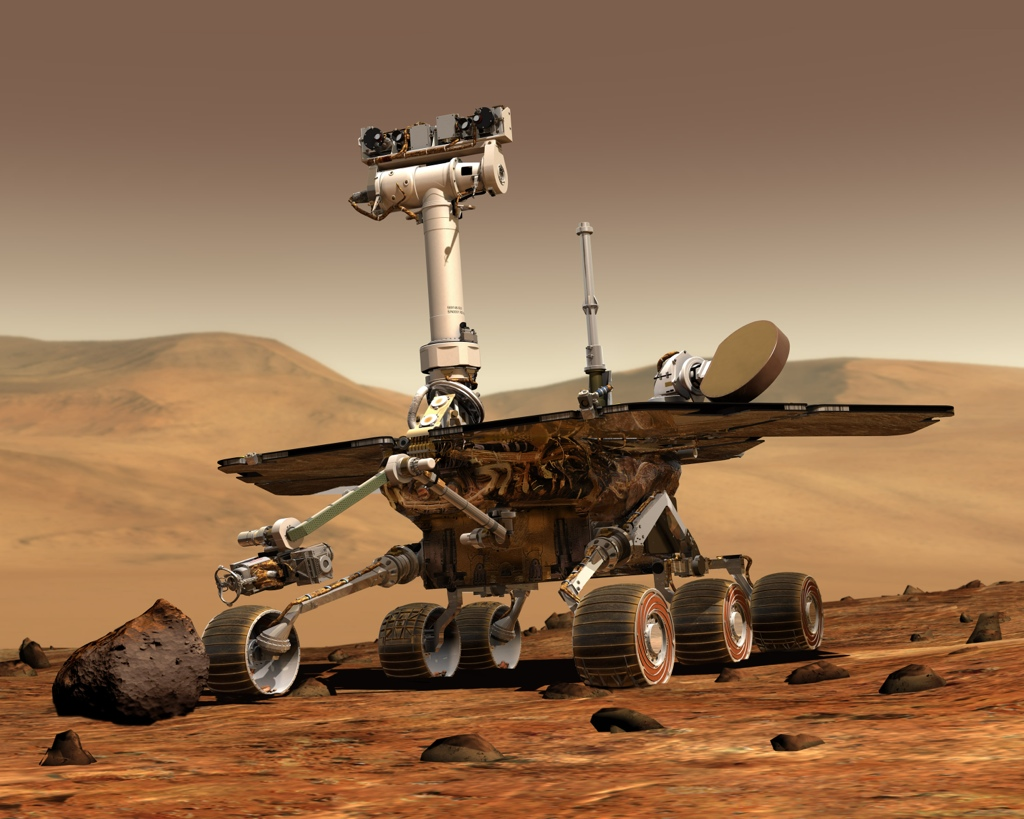
\includegraphics[width=6cm]{kapitel3/nasa_rover}
  \caption{Ein Nasa Rover}
  \label{Kap2:NasaRover}
\end{figure}

Man kann sich auch selbst ein Makro für das Einfügen von Bildern schreiben:

\bild{kapitel3/modell_point_to_point}{6cm}{Point to Point}

\begin{sidewaysfigure}
 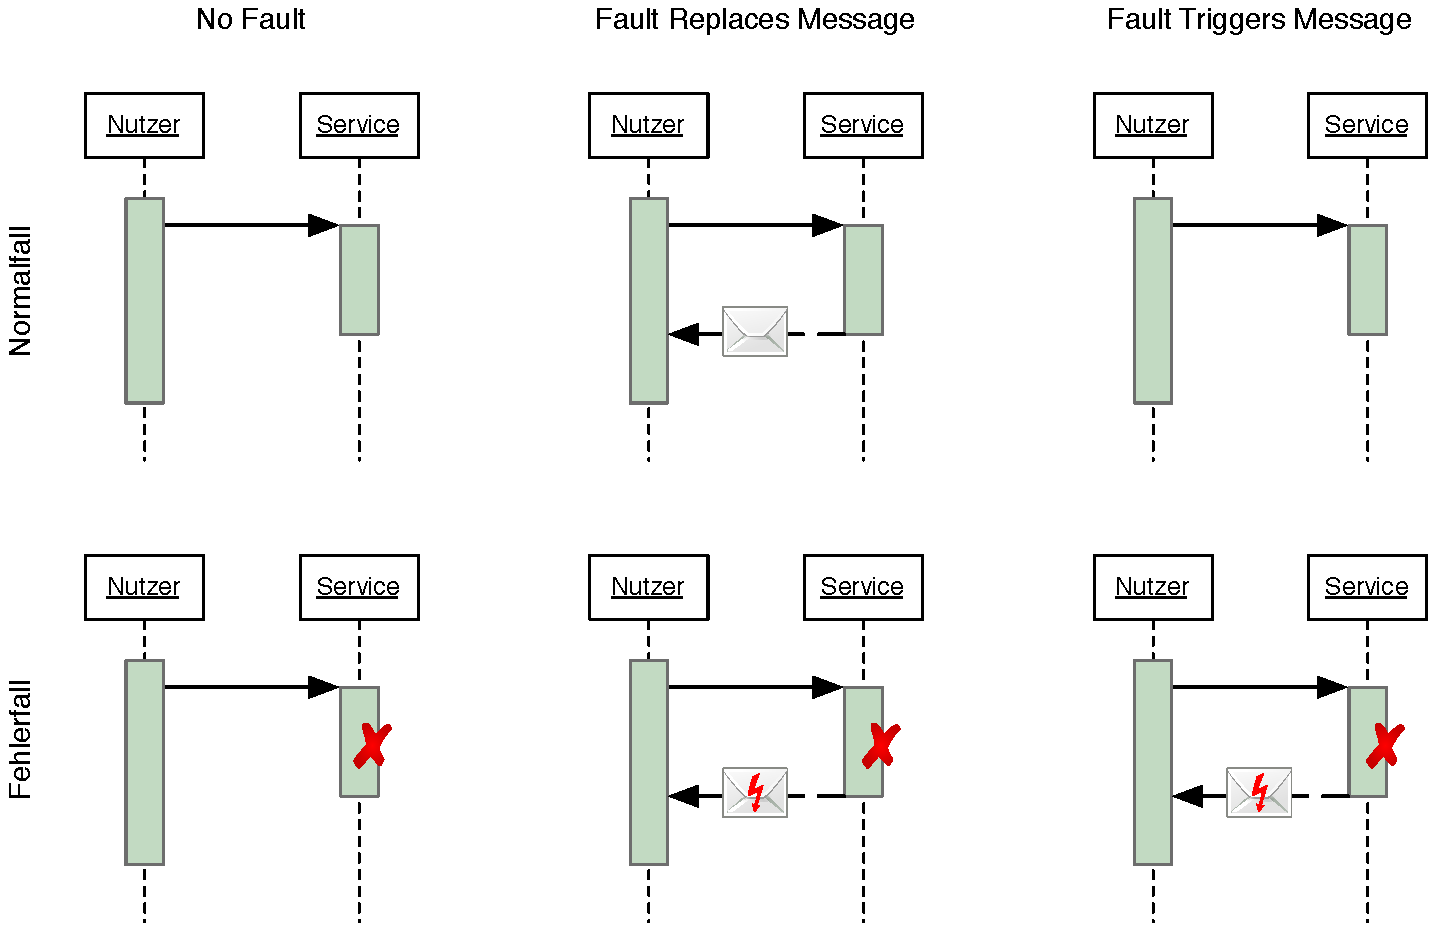
\includegraphics[width=22cm]{kapitel3/ws-wsdl20-fehler}
  \caption{Sehr große Grafiken kann man drehen, damit sie auf die Seite passen}
  \label{Kap2:wsdl-fehler}
\end{sidewaysfigure}

Möchte man verhindern, dass Bilder in ein anderes Kapitel rutschen, steht der Befehl \verb+\clearpage+ zur Verfügung, der \LaTeX{} zwingt, alle bis dahin definierten \textit{floats} (Bilder, Tabellen, Formeln etc.) auszugeben.

\clearpage % Alle Bilder, die bisher kamen ausgeben


\section{Formelsatz}

Eine Formel gefällig? Mitten im Text $a_2 = \sqrt{x^3}$ oder als eigener Absatz (siehe \autoref{Formel}):

\begin{equation}
\begin{bmatrix}
   1 &  4 &  2 \\
   4 &  0 & -3
\end{bmatrix}
        \cdot
\begin{bmatrix}
   1 &  1 &  0 \\
  -2 &  3 &  5 \\
   0 &  1 &  4
\end{bmatrix}
       {=}
\begin{bmatrix}
  -7 &  15 &  28 \\
   4 &   1 & -12
\end{bmatrix}
\label{Formel}
\end{equation}

Wenn Ihre Formel zu breit für eine Zeile wird, können Sie sie mithilfe der \texttt{split}-Umgebung und einem doppelten Backslash (\verb+\\+) umbrechen.

\begin{equation}
\label{eq:4}
\begin{split}
\mathbf{F}_{{eigen}}=\sqrt[3]{\coprod_{i=1}^{3} \lambda_{i}},
\frac{\lambda_{1}-\lambda_{3}}{\lambda_{1}},
\frac{\lambda_{2}-\lambda_{3}}{\lambda_{1}},
\frac{\lambda_{3}}{\lambda_{1}} \\-
\sum_{i=1}^{3} \lambda_{i} \log \left(\lambda_{i}\right),
\frac{\lambda_{1}-\lambda_{2}}{\lambda_{1}}
\end{split}
\end{equation}

Sie können Formelelemente auch am Gleichheitszeichen ausrichten, hierzu dient die \texttt{align}-Umgebung:

\begin{align}
2x - 5y &=  8 \\
3x + 92y &=  -12
\end{align}

Wollen Sie keine Nummerierung der Formeln, ergänzen Sie einfach einen \texttt{*} bei den Namen der Umgebungen, d.h. Sie verwenden \texttt{equation*} oder \texttt{align*}.

\begin{equation*}
\begin{bmatrix}
   1 &  4 &  2 \\
   4 &  0 & -3
\end{bmatrix}
        \cdot
\begin{bmatrix}
   1 &  1 &  0 \\
  -2 &  3 &  5 \\
   0 &  1 &  4
\end{bmatrix}
       {=}
\begin{bmatrix}
  -7 &  15 &  28 \\
   4 &   1 & -12
\end{bmatrix}
\end{equation*}


\section{Sourcecode}

Man kann mit Latex auch ganz toll Sourcecode in den Text aufnehmen.

\subsection{Aus einer Datei}

\lstinputlisting[firstline=2,                 % Erste anzuzeigende Zeile aus der Datei
                 language=Java,               % Programmmiersprache (für Highlighting)
                 caption={Crypter-Interface}, % Beschriftung
                 label=lst:CrypterInterface]  % Label (für Referenzen)
                 {\srcloc/Crypter.java}       % Pfad zur Datei, die angezeigt wird

Mit Zeilennummern

\lstinputlisting[numbers=left,                % Mit Zeilennummern auf der linken Seite
                 firstline=10,                % Erste anzuzeigende Zeile aus der Datei
                 lastline=15,                 % Letzte anzuzeigende Zeile aus der Datei
                 language=Java,               % Programmmiersprache (für Highlighting)
                 caption={Crypter},           % Beschriftung
                 label=lst:CrypterInterface2] % Label (für Referenzen)
                 {\srcloc/Crypter.java}       % Pfad zur Datei, die angezeigt wird


\subsection{Inline}

\begin{lstlisting}[language=Java,caption=Methode checkKey()]
    /**
     * Testet den Schlüssel auf Korrektheit: Er muss mindestens die Länge 1
     * haben und darf nur Zeichen von A-Z enthalten.
     *
     * @param key zu testender Schlüssel
     * @throws CrypterException wenn der Schlüssel nicht OK ist.
     */
    protected void checkKey(Key key) throws CrypterException {

        // Passt die Länge?
        if (key.getKey().length == 0) {
            throw new CrypterException("Der Schlüssel muss mindestens " +
                    "ein Zeichen lang sein");
        }

        checkCharacters(key.getKey(), ALPHABET);
    }
\end{lstlisting}


\section{Anforderungen}

Anforderungen im Format des Volere"=Templates (Snowcards) \autocite{Volere} können per Makro eingefügt werden. Das Label wird automatisch mit der Nummer erstellt, d.\,h. Sie können auf die Tabelle mit dieser referenzieren (siehe \autoref{F52}).

\snowcard % Snowcard einbinden (Anpassungen in titelblatt.tex)
   {F52} % Nummer des Requirements
   {F} % Art
   {Hoch} % Priorität
   {User Authentifizierung} % Titel
   {Interview mit Abteilungsleiter} % Herkunft (Optional)
   {F12} % Konflikte (Optional)
   {Der Benutzer ist in der Lage sich über seinen
    Benutzernamen und sein Passwort am System anzumelden} % Beschreibung
   {Ein Benutzer kann sich mit seinem firmenweiten Benutzernamen und
   Passwort über die Anmeldemaske anmelden und hat Zugriff auf die
   Funktionen des Systems} % Fit-Kriterium (Optional)
   {Benutzerhandbuch des Altsystems} % Material (Optional)

Ebenso können Sie nicht"=funktionale Anforderungen mit Hilfe von Quality Attribute Scenarios (vgl. \autoref{NF11}) darstellen. Zu Details siehe \autocite{Barbacci2003}.

\qas % Quality-Attribute Scenario einbinden (Anpassungen in titelblatt.tex)
   {NF11} % Nummer des Requirements
   {Hoch} % Priotität
   {Performance des Jahresabschlusses} % Titel
   {Endbenutzer} % Quelle
   {Startet einen Jahresabschluss} % Stimulus
   {Buchhaltungssystem} % Artefakt
   {Das System befindet sich im normalen Betriebszustand} % Umgebung
   {Jahresabschluss ist durchgeführt und kann als PDF abgerufen werden} % Antwort
   {10 Minuten} % Antwort-Maß

Die Abgrenzung von funktionalen und nicht-funktionalen Anforderungen ist nicht immer einfach und bereitet manchen Studierenden Probleme. Als Hilfestellung kann die von der ISO25010 \autocite{ISO25010} zur Verfügung gestellte Liste dienen, siehe \autoref{kapitel3/iso25010}.

\bild{kapitel3/iso25010}{14cm}{Qualitätsmodell für Software-Produkte nach ISO25010}

\citeauthor{Bass2003} listen in \autocite{Bass2003} eine ähnliche Liste von Kategorien für nicht-funktionalen Anforderungen auf, die ebenfalls als Richtschnur dienen kann. Diese sind:

\begin{itemize}
  \item \textit{Verfügbarkeit} \textit{(availability)} -- umfasst Zuverlässigkeit (reliability), Robustheit (robustness), Fehlertoleranz (fault tolerance) und Skalierbarkeit (scalability)
  \item \textit{Anpassbarkeit} \textit{(modifiability)}, umfasst Wartbarkeit (maintainability), Verständlichkeit (understandability) und Portabilität (portability).
  \item \textit{Performanz} \textit{(performance)}
  \item \textit{Sicherheit} \textit{(security)}
  \item \textit{Testbarkeit} \textit{(testability)}
  \item \textit{Bedienbarkeit} \textit{(usability)}
\end{itemize}
 % Externe Datei einbinden
% \chapter{Checkliste}
\label{Kap4}

Die folgende Checkliste kann dazu dienen, die Arbeit auf die wichtigsten Bewertungskriterien zu prüfen. Jeder Dozent hat andere Kriterien, die unten aufgeführten dürften aber für die meisten Dozenten gültig sein.

\section{Form und Sprache}

\begin{checklist}
  \footnotesize
  \item \textbf{Aufbau}: Die Arbeit ist nach wissenschaftlichen Prinzipien aufgebaut (wesentliche Teile vorhanden, Nummerierung/Verweise korrekt, Verzeichnisse vorhanden).
    \begin{checklist}
        \item \textit{Wesentliche Teile}: Die folgenden Elemente der Arbeit sind vorhanden: Titelblatt, Abstract/Zusammenfassung, Einleitung, Hauptteil, Fazit/Ausblick.
        \item \textit{Nummerierung/Verweise}: Das Nummerierungsschema wird konsistent über die gesamte Arbeit durchgehalten, die Verweise auf die verschiedenen Elemente (Abbildungen, Tabellen etc.) sind korrekt.
        \item \textit{Verzeichnisse}: Die Arbeit enthält alle relevanten Verzeichnisse: Inhaltsverzeichnis, Literaturverzeichnis, Abbildungsverzeichnis, Tabellenverzeichnis, eventuell Glossar.
    \end{checklist}
  \item \textbf{Sprache}: Die verwendete Sprache entspricht wissenschaftlichen Ansprüchen.
    \begin{checklist}
        \item \textit{Begriffe und Definitionen}: Begriffe werden einheitlich und konsistent verwendet. Neue Begriffe werden definiert und mit Literatur hinterlegt.
        \item \textit{Abkürzungen}: Alle Abkürzungen werden eingeführt und erläutert. Abkürzungen werden bei der ersten Verwendung ausgeschrieben und in einem Abkürzungsverzeichnis geführt. Es werden keine unüblichen oder selbst erfunden Abkürzungen verwendet. Ein Glossar kann verwendet werden, um Begriffe noch einmal kompakt darzustellen.
        \item \textit{Rechtschreibung}: Die Arbeit ist frei von Rechtschreibungs-, Zeichensetzungs- und Grammatikfehlern.
    \end{checklist}
  \item \textbf{Formatierung, Typografie}: Die Formatierung der Arbeit ist korrekt und aus typographischer Sicht einwandfrei. \textit{Wenn Sie dieses Template korrekt verwenden, sollte dieser Punkt automatisch durch die Verwendung von \LaTeX \ erledigt sein.}
    \begin{checklist}
        \item \textit{Korrekte Typografie}: Schriftarten werden korrekt verwendet (nicht mehr als 2 Fonts), der Zeilenabstand ist passend, die Ränder sind ausreichend, der Satz ist korrekt.
        \item \textit{Satz von Abbildungen, Tabellen etc.}: Abbildungen sind in der richtigen Auflösung dargestellt, die Tabellen sind korrekt gesetzt, mathematische Formeln und Symbole sind sauber dargestellt.
    \end{checklist}
  \item \textbf{Abbildungen}: Abbildungen werden in ausreichendem Umfang zur Förderung des Verständnisses eingesetzt. Sie werden korrekt im Text referenziert und sind, wo immer möglich, in einer Standardnotation erstellt.
    \begin{checklist}
        \item \textit{Ausreichende Verwendung}: Komplizierte Sachverhalte werden durch Abbildungen verdeutlicht. Es werden genug Abbildungen eingesetzt, um die wichtigsten Sachverhalte zu erklären.
        \item \textit{Verständnisförderung}: Abbildungen dienen nicht als Schmuck, sondern um komplizierte Sachverhalte zu verdeutlichen.
        \item \textit{Einbindung in den Text}: Der Text muss auch ohne Abbildungen verständlich sein, die Abbildungen helfen Sachverhalte aus dem Text besser darzustellen. Der Text referenziert die Abbildung korrekt.
        \item \textit{Standardnotation, Legende}: Die Abbildungen verwenden Standard"=Notationen wie UML, FMC etc. Wo keine Standardnotation eingesetzt wird, ist eine Legende vorhanden, um die Bildelemente zu erläutern.
    \end{checklist}
  \item \textbf{Zitate}: Quellen werden konsistent nach einer gängigen Zitierweise zitiert und sind vollständig im Literaturverzeichnis angegeben.
    \begin{checklist}
        \item \textit{Zitierweise}: Die Zitierweise in der gesamten Arbeit folgt einem einheitlichen Schema, z.B. IEEE, DIN, Chicago.
        \item \textit{Vollständigkeit}: Alle Zitate sind als solche kenntlich gemacht und die Quelle wird vollständig angegeben, und Plagiate werden vermieden.
    \end{checklist}
  \item \textbf{Schreibstil}: Lebendiger, wissenschaftlicher und verständlicher Schreibstil.
    \begin{checklist}
        \item \textit{Wissenschaftlichkeit}: Der Text ist im Präsenz geschrieben, es wird die dritte Person verwendet, Fachausdrücke werden korrekt verwendet, Fremdwörter und Amerikanismen werden richtig eingesetzt.
        \item \textit{Verständlichkeit}: Abschweifungen und Wiederholungen werden vermieden, statt dessen werden präzise und übersichtliche Sätze verwendet.
        \item \textit{Lebendigkeit}: Der Text der Arbeit zeichnet sich durch eine gute Wortwahl, Sprachbilder, einen angemessenen Satzbau und eine hohe Variabilität aus.
    \end{checklist}
\end{checklist}

\section{Inhalt}

\begin{checklist}
  \footnotesize
  \item \textbf{Gliederung}: Die Gliederung ist vollständig, konsistent und sachlogisch mit angemessener Struktur und Tiefe.
    \begin{checklist}
        \item \textit{Konsistenz und Vollständigkeit}: Auf einer Ebene stehen keine Punkte alleine, die Gliederungspunkte orientieren sich an der Argumentationskette.
        \item \textit{Angemessene Tiefe}: Die Größe der einzelnen Unterpunkte ist vom Umfang her ähnlich. Es gibt keine Gliederungspunkte, die nur aus ein bis zwei Sätzen bestehen.
    \end{checklist}
  \item \textbf{Grundlagen}: Es werden alle relevanten Grundlagen gelegt. Der State"=of"=the"=art und der State"=of"=practice werden dargelegt.
    \begin{checklist}
        \item \textit{Umfang}: 1/3 des Hauptteils ist ein gutes Maß für eine ausreichende Darstellung der Grundlagen.
        \item \textit{Begriffe und Methoden}: Begriffe und Methoden sind definiert, und Literatur zu den Definitionen ist angegeben.
        \item \textit{State-of-the-art}: Der Stand des verfügbaren Wissens wird dargestellt, analysiert und kritisch beurteilt (state-of-the-art). Bei theoretischen Arbeiten kann ein eigenes Kapitel \enquote{verwandte Arbeiten} nötig sein, um den state"=of"=the"=art darzustellen.
        \item \textit{State-of-practice}: Bei praktischen Arbeiten, die in der Industrie geschrieben werden, kann es nötig sein, auch das Vorgehen im Unternehmen zu erläutern.
    \end{checklist}
  \item \textbf{Methodik/Lösung}: Die gewählte Methodik bzw. Lösung ist für das Problem adäquat.
    \begin{checklist}
        \item \textit{Anforderungen an die Lösung}: Die von der Lösung zu erfüllenden Anforderungen werden dargestellt. Wo nötig wird dies auf Grundlage eines sauberen Requirements"=Engineerings durchgeführt.
        \item \textit{Erläuterung des Lösungsansatzes}: Der gewählte Lösungsansatz wird ausführlich erläutert und verständlich dargestellt.
        \item \textit{Eignung zur Lösung der Aufgabe}: Die gewählte Lösung ist geeignet, um das beschriebene Problem zu lösen.
        \item \textit{Hypothesen}: Es sind ggf. Hypothesen gebildet worden; diese sind erläutert, und es sind Kriterien identifiziert worden, mit deren Hilfe man die Hypothesen falsifizieren kann.
        \item \textit{Alternativen}: Es werden Alternativen zur vorgeschlagenen Lösung diskutiert. Die eigene Lösung wird nicht als einzige mögliche dargestellt, sondern es werden auch andere mögliche Lösungen vorgestellt und bewertet.
        \item \textit{Begründung}: Alternativen und Kriterien für die Auswahl dieser Lösung werden dargestellt.
        \item \textit{Vorteile der Lösung}: Es wird dargestellt, wieso die entwickelte Lösung vorteilhafter ist als die bisherigen Ansätze. Diese Darstellung erfolgt auf Basis des Lösungsansatzes. Eine konkrete Validierung der Implementierung erfolgt ggf. in späteren Kapiteln.
    \end{checklist}
  \item \textbf{Logik der Argumentationskette}: Die Argumentation ist logisch und nachvollziehbar. Sie ist frei von logischen Fehlschlüssen.
  \item \textbf{Implementierung}: Wenn eine Implementierung der Lösung erfolgt, so wird die Implementierung beschrieben. Die Darstellung der Implementierung kann knapp ausfallen. Wichtig ist der Lösungsansatz, nicht die konkrete Umsetzung.
  \item \textbf{Validierung}: Die vorgeschlagene Lösung wird ggf. empirisch verprobt.
    \begin{checklist}
        \item \textit{Vorgehensweise}: Die Vorgehensweise zur Validierung der Lösung / Hypothesen ist beschrieben und geeignet, relevante Aspekte der Lösung zu überprüfen.
        \item \textit{Empirische Analyse}: Die Erfassungsmethode wird dargestellt und die Daten werden nach den Grundsätzen ordnungsgemäßer Laborpraxis gesammelt und statistisch korrekt ausgewertet.
        \item \textit{Verprobung}: Die Lösung wird an einem praktischen Beispiel verprobt, und es werden wissenschaftlich korrekte Schlüsse aus der Anwendung gezogen.
        \item \textit{Zielerreichung}: Funktioniert die gewählte Lösung nach der Implementierung? Wie weit wurde das Ziel erreicht? Falls nicht, gibt es nachvollziehbare Gründe dafür und wurden diese dargestellt?
    \end{checklist}
  \item \textbf{Diskussion}: Die Lösung und ihre Validierung wird kritisch und im Kontext möglicher Alternativen diskutiert und bewertet.
    \begin{checklist}
        \item \textit{Kritische Reflexion}: Grenzen und Schwächen der eigenen Ergebnisse werden beleuchtet.
        \item \textit{Ableitung von Konsequenzen}: Die Konsequenzen aus den Ergebnissen für die Wissenschaft und Praxis sind beschrieben.
    \end{checklist}
  \item \textbf{Quellenarbeit}: Es werden hochwertige Quellen in ausreichendem Umfang genutzt und kritisch hinterfragt. Eventuell vorhandene Quellen aus dem Unternehmen werden ebenfalls berücksichtigt.
    \begin{checklist}
        \item \textit{Umfang}: Der Umfang an Quellen richtet sich stark nach Thema und Art der Arbeit. Bei einer Bachelorarbeit sind mindestens 20--30 Quellen üblich, bei einer Masterarbeit deutlich mehr.
        \item \textit{Wissenschaftliche Qualität}: Nicht zitierfähig sind Internet"=Quellen, Wikipedia"=Einträge sowie andere Bachelor- oder Masterarbeiten (sofern nicht veröffentlicht). Das ausschließliche Zitieren von Lehrbüchern ist problematisch. Aktuelle wissenschaftliche Artikel und Werke sollten in den Quellen auftauchen.
        \item \textit{Quellen \enquote{aus der Praxis}}: Wenn es im Unternehmen spezielle Quellen und Informationen gibt, so werden diese berücksichtigt, z. B. firmen- oder branchenspezifischer Informationen.
        \item \textit{Kritische Würdigung}: Quellen und Zitate werden kritisch hinterfragt und nicht einfach unreflektiert übernommen. Es gibt eine kritische Distanz bei der Quellenauswahl und Quellenauswertung.
    \end{checklist}
  \item \textbf{Fazit}: Es wird eine Zusammenfassung der Arbeit sowie Ausblick auf weitere mögliche Arbeiten im Themenfeld gegeben, etwa die Lösung ausstehender Probleme oder die Erfüllung zusätzlicher Anforderungen.
  \item \textbf{Umfang der Arbeit}: Richtgrößen: Bachelorarbeiten: 50--80 Seiten, Masterarbeiten: 60--100 Seiten, jeweils ohne Verzeichnisse und Anhang.
\end{checklist}

\section{Vor der Abgabe}

\begin{checklist}
  \footnotesize
  \item \textit{Korrektur}: Haben Sie einen Dritten die Arbeit lesen lassen und alle gefundenen Rechtschreib- und Zeichensetzungsfehler behoben?
  \item \textit{Literaturverzeichnis}: Sind im Literaturverzeichnis irrelevante Informationen entfernt? Beispielsweise bei Büchern unnötige Informationen über die Herkunft bei Google-Books oder bei Papern doppelte Angaben der DOI?
  \item \textbf{Abgabe auf Papier}
  \begin{checklist}
    \item \textit{Template passend eingestellt}: Haben Sie in der Datei \texttt{thesis.tex} eingestellt, dass Sie auf Papier abgeben wollen?
    \item \textit{Doppel- oder einseitiger Druck}: Entspricht die Einstellung des Templates dem Druck, d.\,h. ist das Template für doppelseitigen Druck eingestellt, wenn doppelseitig gedruckt werden soll und umgekehrt?
    \item \textit{Umschläge}: Sind die Umschläge vorhanden, um die Arbeit später zu binden? Die Umschläge können in der Hausdruckerei der Hochschule erworben werden.
    \item \textit{Copyshop}: Wissen Sie, wo Sie die Arbeit drucken werden? Die Hausdruckerei kann Ihre Arbeit nicht drucken.
    \item \textit{Exemplare}: Haben Sie geklärt, ob der Zweitkorrektor auch ein gedrucktes Exemplar möchte?
  \end{checklist}
  \item \textbf{Digitale Abgabe}
  \begin{checklist}
    \item \textit{Zustimmung des Betreuers/der Betreuerin}: Haben Sie mit Ihrer Betreuerin bzw. Ihrem Betreuer abgeklärt, dass Sie digital abgeben dürfen?
    \item \textit{Template passend eingestellt}: Haben Sie in der Datei \texttt{thesis.tex} eingestellt, dass Sie digital abgeben wollen?
    \item \textit{Unterschrift}: Haben Sie Ihre Unterschrift eingescannt und unter dem Namen \texttt{unterschrift.png} im Hauptverzeichnis abgelegt?
  \end{checklist}
\end{checklist}
 % Externe Datei einbinden
\chapter{Einleitung}

Computerschach ist ein viel betrachtetes Thema. Schon Alan Turing und Claude Shannon haben sich damit befasst \cite{Turing1953, Shannon1950}. In seinem \citeyear{Shannon1950} verfassten Paper beschrieb \citeauthor{Shannon1950} \cite{Shannon1950} die Funktion zu Evaluation einer Schachposition. Ihm war jedoch auch klar, dass es wahrscheinlich niemals eine exakte Evaluation für Schach geben wird. Deshalb liegt es nahe, dafür ein \ac{NN} zu verwenden, denn dessen Aufgabe ist es, eine solche Funktion zu approximieren. Leider ist es für die Evaluation in einem Schachcomputer wichtig, sowohl genau als auch schnell die Position zu bewerten. Je genauer die Stellung bewertet wird, desto stärker spielt das Programm. Je schneller die Bewertung stattfindet, desto weiter kann der Computer voraussehen, was ebenfalls zu einer höheren Spielstärke führt. Herkömmliche \acp{NN} Architekturen scheitern jedoch an einer zu lagen Berechnungszeit oder bei sehr kleinen Netzen an einer zu ungenauen Bewertung.

Eine Lösung für die Probleme herkömmlicher \acp{NN} wurde \citeyear{YNasu2018} von \citeauthor{YNasu2018} \cite{YNasu2018} in seinem japanischen Paper vorgestellt. Er erkannte, dass inkrementelle Aktualisierungen, wie sie bereits in \ac{HCE} verwendet wurden, in \acp{NN} verwendet werden können. Der Schlüssel dafür ist ein binäres und dünn besetztes Feature Set, basierend auf den Figuren und ihren Positionen. Die Eingabeschicht, auch affiner Transformator genannt, muss nicht bei jeder Aktivierung alle Elemente seines Ausgabevektors neu berechnen.

Die \ac{NNUE} Architektur ist darauf ausgelegt, schnell auf einer CPU zu laufen. Sie nutzt CPU-basierte Optimierungsmöglichkeiten wie \ac{SIMD} und die im letzten Absatz genannten inkrementellen Aktualisierungen, um die Geschwindigkeit zu erlangen und ihre Nutzung als Evaluationsfunktion zu rechtfertigen.

\citeauthor{YNasu2018}s \cite{YNasu2018} hat die \ac{NNUE} Architektur für die Verwendung in der japanischen Schachvariante Shogi entwickelt. Shogi unterscheidet sich in einigen Punkten vom herkömmlichen Schach. Es hat unter anderem eine andere Spielfeldgröße und erlaubt es, geschlagene Figuren wieder einzusetzen. Trotzdem eignet sich \citeauthor{YNasu2018}s \cite{YNasu2018} Ansatz für traditionelles Schach, da die Zuggenerierung sowie die Evaluation ähnlich ist. Außerdem gibt es in beiden Varianten einen König, praktisch für die Auswahl eines passenden Feature Sets, wie in \autoref{chap:featureSet} genauer erläutert.

Nur zwei Jahre später zeigte eine Portierung des Konzepts starke Verbesserungen in dem Schachcomputer Stockfish, der sich durch \ac{NNUE} um mehr als 80 Elo verbessern konnte \cite{StockfishIntroducingNNUE}, die größte Verbesserung einer Stockfish-Version jemals. Mit Ausnahme von AlphaZero \cite{Silver2017} hatte bis dahin noch kein \ac{NN} basierter Ansatz Erfolge gezeigt.

% mMtivation für Schachcomputer beschreiben:
% warum ist Schach eine gute Spielweise für Computer Scientist (DeepMind)
% warum werden normale Schachspieler besser durch bessere/andere Schachcomputer (besonders welche mit Neuronalem Netz)

Ein Schachcomputer besteht aus drei Teilen: Suche, Zuggenerierung (Boardrepräsentation) und Evaluation \cite{VazquezFernandez2013}. Als Basis für diese Arbeit wird ein simpler Schachcomputer, der in dem Modul \ac{KIS} entwickelt wurde, verwendet. Dieser Schachcomputer verfügt über eine simple Suche und eine \ac{HCE} \cite{nopy}. Gegenstand dieser Arbeit ist es, die \ac{HCE} des 2021 im Modul \ac{KIS} entwickelten Schachcomputers durch ein eigens trainiertes \ac{NNUE} zu ersetzen. Ziel ist es hierbei nicht, eine neue \ac{NNUE} Architektur zu präsentieren. Es wird die Architektur verwendet, die von \citeauthor{YNasu2018} \cite{YNasu2018} vorgestellt und auch in der ersten Version der Stockfish \ac{NNUE} verwendet wurde. Der Grund dafür ist, dass sie mit minimalem Domänenwissen auskommt und so ein besseres Bild der Kernelemente der \ac{NNUE} Architektur vermittelt. Außerdem sollte sie, gemessen an dem Erfolg in Stockfish, ausreichen, um die Spielstärke des in \ac{KIS} entwickelten Schachcomputers zu steigern.
Die \ac{NNUE} Implementierung soll ein Proof of Conzept sein. Die Erstellung neuer Eingabedaten für \acp{NNUE} ist nicht Teil dieser Arbeit.
\chapter{Grundlagen}

In diesem Kapitel wird das Wissen vermittelt, welches benötigt wird, um zu verstehen, wie \acp{NNUE} im Rahmen von Schachcomputern funktionieren. Zuerst wird die Evaluation, wie sie in herkömmlichen Schachcomputern funktioniert, erklärt, auch \ac{HCE} genannt. Weiterhin wird auf die grundlegenden Bestandteile, die für überwacht lernende \acp{FNN} von Bedeutung sind, eingegangen. Außerdem wird erläutert, was \ac{SIMD} ist und wie diese Vektoroperationen in C/C++ verwendet werden können. Zuletzt wird die grundlegende Funktionsweise von \acp{NNUE} vermittelt, die auf den davor gelegten Grundsteinen aufbaut.

\section{Hand-crafted Evaluation}
\label{chap:HCE}

Es ist wichtig zu wissen, wie die \ac{HCE} eines Schachcomputers funktioniert, da sie nicht nur die Variante ist, die in jedem starken Schachcomputer vor 2017 eingesetzt wurde, sondern auch heute noch in Kombination mit \ac{NNUE} eingesetzt wird. Bei \ac{NNUE}-Schachcomputern wird sie oft in Kombination mit der \ac{NN}-Evaluation genutzt, weil sie besser in extremen Stellungen funktioniert. Besitzt beispielsweise weiß in einer Position eine Dame mehr, muss nicht die teurere Berechnung des \acp{NNUE} durchgeführt werden, um zu entscheiden, dass Weiß im Vorteil ist.

Die \ac{HCE} einer Schachposition ist eine heuristische Methode der Position einen numerischen Wert zuzuordnen. Vor der Verbreitung von \acp{NN} war \ac{HCE} die einzige Form der Positions-Evaluation. Gäbe es unendliche Ressourcen, könnten aus jeder Position alle möglichen Zugfolgen per Brute Force bestimmt und den Positionen einer der drei Werte: -1 (Verlust), 0 (remis), 1 (Gewinn) gegeben werden. In der Realität ist es nicht möglich, den exakten Wert der Stellung zu kennen. Deshalb wird in der \ac{HCE} versucht, anhand von Menschen festgelegten Kriterien der Position einen Wert zuzuordnen. Die so gewonnene Bewertung wird in der Zugsuche verwendet, um den besten Zug, abhängig von den per Hand gewählten Kriterien, zu finden. Die Evaluation wird aus Sicht der Seite, die gerade am Zug ist, angegeben. Das ist wichtig für den verwendeten Suchalgorithmus (Alpha-Beta-Suche) \cite{Slagle1969}.

Die \ac{HCE} eines Schachcomputers ähnelt in einigen Aspekten mehr einer Philosophie als einer Funktion. Schach ist ein Spiel, das es seit über 1000 Jahren gibt. In dieser Zeit haben Menschen Regeln überlegt, um besser Schach zu spielen. All diese Regeln in die Evaluationsfunktion zu integrieren, ist nicht ratsam. Es ist ein Abwägen zwischen Wissen und Geschwindigkeit. Je mehr Regeln dem Computer gegeben werden, umso weniger weit kann er vorausschauen.

Wenn ein Mensch Schach spielen lernt, ist der Wert der Figuren eines der ersten Erkenntnisse. Das ist ebenfalls der wichtigste Faktor für einen Schachcomputer, wie schon \citeauthor{Shannon1950} \citeyear{Shannon1950} \cite{Shannon1950} erkannte. Die Angabe der Materialwertung wird bei Computern als Centipawn angegeben, um so mehr Spielraum für feingranulare Faktoren zu lassen. Figuren werden ebenfalls anhand ihrer Position bewertet. Dafür gibt es sogenannte Piece Square Tables, die jeder Figur abhängig von ihrer Position einen Wert zuordnen. Beispielsweise ist ein Springer am Rand des Brettes deutlich weniger wert als einer im Zentrum, auch bekannt als \enquote{ein Springer am Rand bringt Kummer und Schand}. Weitere nennenswerte Aspekte der \ac{HCE} sind die Mobilität und Schwachstellen \cite[S. 228]{Levy1988}.

% weitere evlauations aspekte: Mobilität und Schwachstellen
Mobilität beschreibt die Beweglichkeit der Figuren. Sie kann aus der Anzahl der Felder, auf die eine Figur ziehen kann, berechnet werden. Das ist unbrauchbar, weil unbeschützte Felder und die Felder gefesselter Figuren nicht Teil der Mobilität sein sollten \cite[S. 228]{Levy1988}. Mit Schwachstellen sind ungeschützte Figuren, die Sicherheit des Königs, Probleme in der Bauernstruktur und Figuren, die höherwertige Figuren angreifen, gemeint \cite[S. 228]{Levy1988}.

% erklären warum verschiedene Spielphasen eine Rolle spielen
Viele der \ac{HCE}-Aspekte profitieren von einer Differenzierung verschiedener Spielphasen. Schach lässt sich in drei Spielphasen teilen: die Eröffnung, das Mittelspiel und das Endspiel \cite[S. 8]{Levy1988}. Beispielsweise ist es sinnvoll, den Wert der Figuren an die aktuelle Spielphase anzupassen. Ein Bauer im Endspiel ist mehr wert als in der Eröffnung. Zwischen den verschiedenen Phasen wird meist durch die Anzahl der Figuren unterschieden. Da zwischen zwei ähnlichen Stellungen, die in zwei unterschiedlichen Phasen sind, kein großer Unterschied durch den Phasenwechsel entsteht, ist es sinnvoll einen Wert für beide Phasen zu berechnen und dazwischen zu interpolieren.

\section{Neuronale Netze}

\begin{figure}
  \centering
  % inspired by: https://tex.stackexchange.com/questions/153957/drawing-neural-network-with-tikz
  \begin{tikzpicture}[x=2cm, y=1.5cm, >=stealth]
    \tikzstyle{neuron}=[draw,shape=circle,minimum size=1.15cm]
    % draw nerons
    \foreach \m/\l [count=\y] in {1,2,3}
    \node [neuron] (input-\m) at (0,2-\y) {};

    \foreach \m [count=\y] in {1,2,3,4}
    \node [neuron] (hidden-\m) at (2,2.5-\y) {};

    \foreach \m [count=\y] in {1,2}
    \node [neuron] (output-\m) at (4,1.5-\y) {};
    % draw lines  
    \foreach \i in {1,2,3}
    \foreach \j in {1,2,3,4}
    \draw [->] (input-\i) -- (hidden-\j);

    \foreach \i in {1,2,3,4}
    \foreach \j in {1,2}
    \draw [->] (hidden-\i) -- (output-\j);

    \foreach \l [count=\x from 0] in {Eingabeschicht, Versteckte Schicht, Ausgabeschicht}
    \node [align=center, above] at (\x*2,2) {\l};
  \end{tikzpicture}
  \caption{Ein einfaches \acl{NN}}
  \label{fig:beispiel-nn}
\end{figure}

\Acp{KNN} oder einfach \acp{NN} genannt sind Computersysteme, die dem biologischen Vorbild des Gehirns nachempfunden sind. Analog zu seinem biologischen Vorbild besteht ein \ac{NN} aus Neuronen, die miteinander vernetzt sind. Jedes Neuron reagiert auf eingehende Signale mit einer bestimmten Reaktion. Diese Reaktion kann sich durch neu gewonnene Erfahrungen anpassen und ermöglicht, zukünftig besser zu reagieren.

% erklären wie der generelle Aufbau ist
In Abbildung \autoref{fig:beispiel-nn} ist ein einfaches \Acl{NN} zu sehen. Es besteht aus drei Schichten. Die erste Schicht, die Eingabeschicht, nimmt Eingabedaten entgegen. Eingabedaten können ganz unterschiedliche Daten repräsentieren. Ist der Eingabedatensatz beispielsweise ein 100 × 100 Schwarz-Weiß-Bild, ist dies eine Möglichkeit die Eingaben darzustellen. Die Eingabeschicht besteht dann aus 1000 Neuronen die pro Neuron den Zustand eines Pixels (0 = Weiß, 1 = Schwarz) des Bildes gefüttert bekommen. Die zweite Schicht heißt versteckte Schicht, weil von außen nur die Eingabedaten und das Ergebnis sichtbar ist. Sie empfängt die Informationen der Eingabeschicht, gewichtet sie und gibt sie an die Ausgabeschicht weiter. Die versteckte Schicht kann aus mehreren Schichten bestehen. Ein \ac{NN} mit mehreren versteckten Schichten heißt \ac{DNN}. Die letzte Sicht, die Ausgabeschicht, spiegelt das Ergebnis des \acp{NN} wider. Ein Netz, das versucht Bilder zwischen Hunden und Katzen zu unterscheiden, kann zwei Ausgabeneuronen enthalten, eins für die Wahrscheinlichkeit, dass auf dem gegebenen Bild ein Hund ist und eins für die Wahrscheinlichkeit, dass es eine Katze ist. Ein \ac{NN} kann auch nur ein Ausgabeneuron besitzen, wie \zb{} bei der Evaluation einer Schachposition nötig ist. Die Verbindungen der einzelnen Neuronen stellen deren Zusammenhang dar. Wie stark die Abhängigkeit ist, wird durch Gewichte definiert \cite[S. 2--7]{krawczak2013multilayer}.
% Auswahl der Inputdatenspalten gibt an, wieviele Inputneuronen es gibt, die Anzahl der hidden Neuronen ist "egal" je mehr -> desto besser kann das neuronale Netz lernen kinda, output Neuronen gibt die Anzahl der Klassifikationen an, kann auch nur eins sein (regession)

Es gibt verschiedene Modelle \Aclp{NN}. Für diese Thesis sind lediglich \acp{FNN} relevant. \acp{FNN}-basieren auf dem von \citeauthor{rosenblatt1958perceptron} \cite{rosenblatt1958perceptron} beschriebenen mehrlagigen Perzeptron. Das \ac{FNN} zeichnet sich durch seinen zyklenfreien Aufbau aus. Der Datenfluss führt immer von der Eingabeschicht zur Ausgabeschicht. Das \ac{FNN} gilt als die einfachste Netzwerkarchitektur \cite{Schmidhuber2015}.

In der Praxis, so auch in dieser Arbeit, werden für die Entwicklung Neuronaler Netze Frameworks verwendet. Sie abstrahieren große Teile der Komplexität. Trotzdem ist es wichtig, ihre Funktionsweise zu kennen, um Entscheidungen zu treffen und Probleme zu beheben. In den folgenden Unterabschnitten wird grundlegend auf die Einzelteile Neuronaler Netze eingegangen. Zuerst wird das Neuron beschrieben und wie sich seine Aktivität berechnen lässt. Das Unterkapitel Backpropagation beschreibt wie \acp{NN} lernen können.

\subsection{Das Neuron}
\label{chap:neuron}

\begin{figure}
  \centering
  % inspired by: https://davidstutz.de/illustrating-convolutional-neural-networks-in-latex-with-tikz/
  \begin{tikzpicture}[shorten >=1pt,->]
    \tikzstyle{unit}=[draw,shape=circle,minimum size=1.15cm]

    \node[unit](p) at (2,1){$y$};
    \node(dots) at (-0.25,1){\vdots};

    \draw (0,2.5) node[xshift=-10]{$x_0$} -- node [midway,above] {$w_{0}$} (p);
    \draw (0,1.75) node[xshift=-10]{$x_1$} -- node [midway,above] {$w_{1}$} (p);
    \draw (0,0) node[xshift=-10]{$x_n$} -- node [midway,above] {$w_{n}$} (p);
    \draw (p) -- (3,1) node[xshift=30]{$y := f(\varphi)$};
  \end{tikzpicture}
  \caption{Ein einzelnes Neuron mit seinen Eingabe- und Ausgabekomponenten}
  \label{fig:neuron}
\end{figure}

% Neuronen wie sie im Nervensystems eines Menschen vorhanden sind
Das Neuron ist der elementare Bestandteil eines \acp{NN}. Es wurde \citeyear{McCulloch1943} von \citeauthor{McCulloch1943} \cite{McCulloch1943} eingeführt. Neuronen sind in einem \ac{NN} mit anderen Neuronen verbunden und bilden so beliebig komplexe Funktionen ab. In \autoref{fig:neuron} ist ein einzelnes Neuron zu sehen. Die Eingänge $x_{0}$ bis $x_{n}$ werden mit den Gewichten $w_{0}$ bis $w_{n}$ multipliziert, aufsummiert und mit der Aktivierungsfunktion $f(\varphi)$ aktiviert. Für gewöhnlich ist immer $x_{0}=1$, was ihn zu dem Bias des Neurons mit $w_{0}=b$ macht. Das bedeutet, dass es nur $n$ tatsächliche Eingabewerte gibt: von $x_{1}$ bis $x_{n}$. Konkret lässt sich die Aktivität eines Neurons mit der \autoref{equation:NeuronActivation} und die Ausgabe $y$ mit \autoref{equation:NeuronOutput} bestimmen:

% mathematische Grundlage für das Neuron und Neuronale Netz
\begin{equation}
  f(\varphi) = \varphi(\sum_{i=0}^{n}w_{i}x_{i})
  \label{equation:NeuronActivation}
\end{equation}

\begin{equation}
  y = f(\varphi)
  \label{equation:NeuronOutput}
\end{equation}

\begin{figure}
  \centering
  \begin{subfigure}{.5\textwidth}
    \centering
    \resizebox{.9\textwidth}{!}{%
      \begin{tikzpicture}[declare function={sigma(\x)=1/(1+exp(-\x));}]
        \begin{axis}%
          [
            grid=none,
            xmin=-6,
            xmax=6,
            axis x line=bottom,
            ytick={0,.5,1},
            ymax=1,
            axis y line=middle,
            samples=100,
            domain=-6:6,
            legend style={at={(1,0.9)}}
          ]
          \addplot[blue,mark=none]   (x,{sigma(x)});
        \end{axis}
      \end{tikzpicture}
    }
    \caption{Standardsigmoide Aktivierungsfunktion}
    \label{fig:sigmoid}
  \end{subfigure}%
  \begin{subfigure}{.5\textwidth}
    \centering
    \resizebox{.9\textwidth}{!}{%
      \begin{tikzpicture}[declare function={relu(\x)=max(0,\x);}]
        \begin{axis}%
          [
            grid=none,
            xmin=-3,
            xmax=3,
            axis x line=bottom,
            ytick={0,1,2,3},
            ymax=3,
            axis y line=middle,
            samples=1000,
            domain=-3:3,
            legend style={at={(1,0.9)}}
          ]
          \addplot[blue,mark=none]   (x,{relu(x)});
        \end{axis}
      \end{tikzpicture}
    }
    \caption{Rectified linear Aktivierungsfunktion}
    \label{fig:Relu}
  \end{subfigure}
  \caption{Beispiele für Aktivierungsfunktionen}
  \label{fig:activationfunction}
\end{figure}

% activation functions: linear vs non linear -> linear Functions sorgen dafür, dass nur ein hidden Layer sinnvoll ist, mehrere hidden Layer mit linearen Aktivierungsfunktionen geben keinen Sinn, da sie zu einer Schicht vereinfacht werden können. Deshalb sind nicht-lineare Transferfunktionen interessant, sie ermöglichen es, komplexere Funktionen zu lernen
Die Aktivierungsfunktion, oder auch Transferfunktion, eines Neurons kann linear oder nicht linear sein. Ist die Transferfunktion linear, ergibt ein mehrschichtiges \ac{NN} keinen Sinn, da sie zu einer Schicht vereinfacht werden können. Außerdem sind lineare \acp{NN} nicht in der Lage, nicht lineare Probleme zu lösen \cite{minsky1969perceptron}. Nicht lineare Transferfunktionen sind interessanter, da sie für nicht lineare Probleme Antworten liefern.

% eingehen auf clipped relu und sigmoid Aktivation Functions
In \autoref{fig:activationfunction} sind zwei Aktivierungsfunktionen zu sehen. In \autoref{fig:sigmoid} ist eine Standardsigmoide abgebildet. Sie sorgt dafür, dass die Ausgabe des Neurons immer zwischen null und eins ist. Berechnet wird sie mit \autoref{equation:sigmoid}. \autoref{fig:Relu} zeigt eine \ac{ReLU}-Transferfunktion. Der niedrigste Wert ist mindestens null. Konkret ist die Berechnung in \autoref{equation:ReLU} angegeben. \ac{ReLU} geht bis ins Unendliche. Wegen der aggressiven Quantisierung muss der Bereich der Aktivierungsfunktionen auch nach oben begrenzt werden, auch Clipped\ac{ReLU} (siehe \autoref{equation:ClippedReLU}) genannt \cite{StockfishNNUE}.

\begin{equation}
  Sigmoid(x)=\frac{1}{(1+e^{-x})}
  \label{equation:sigmoid}
\end{equation}

\begin{equation}
  ReLU(x)=max(0,x)
  \label{equation:ReLU}
\end{equation}

\begin{equation}
  ClippedReLU(x)=min(max(0,x),1)
  \label{equation:ClippedReLU}
\end{equation}


\subsection{Backpropagation und Gradientenabstieg}
\label{chap:bpGradient}
% viel muss man davon nicht kennen, da Pytorch das übernimmt (automatic through automatic differentiation)
Das Besondere an \acp{NN} ist, dass sie lernen, also nach und nach besser werden. Für gewöhnlich wird erwartet, dass ein Programm auf einer Eingabe immer dasselbe Ergebnis liefert. Ein \ac{NN} hingegen lernt während seiner Trainingsphase aus Fehlern. Es gilt, den Fehler zu minimieren. Dabei handelt es sich um ein Optimierungsproblem. Als Lösung dafür wird der Gradientenabstieg verwendet. Es gibt dafür auch andere Methoden, auf die hier nicht weiter eingegangen wird \cite{StockfishNNUE}.

Der Gradientenabstieg minimiert den Fehler, indem er dem negativen Gradienten einer Verlustfunktion folgt \cite{Ruder2016}. Die Annahme ist, dass die Richtung des Gradienten einer Funktion diese maximiert. Deshalb führt ein Schritt in die entgegengesetzte Richtung zu einer Minimierung der Funktion, also einer Minimierung des Fehlers. Die Lernrate steuert die Schrittweite, die dem negativen Gradienten folgt. Sind die Schritte zu groß, wird das (lokale) Minimum übersprungen. Sind sie klein, dauert die Konvertierung länger oder bleibt in einem lokalen Minimum hängen. Um beide dieser Probleme bestmöglich zu vermeiden, ist die Lernrate nicht konstant, sondern ändert sich über den Trainingszeitraum.

Die Lernrate kann entweder abhängig durch einen festen Plan oder durch ein adaptives Modell angepasst werden. Ein Beispiel für eine fest geplante Änderung ist die Multiplikation der Lernrate mit einem Faktor $x$ alle $n$ Epochen. Eine Epoche ist normalerweise ein Durchgang des gesamten Eingabedatensatzes. Alternativ gibt es verschiedene adaptive Lernraten-Modelle. In dieser Arbeit wird \zb{} Adadelta verwendet. Adadelta ist eine Adaption des Gradientenabstiegs. Diese Variante erweitert den Gradientenabstieg um eine dynamische Lernrate, die akkumulierende Gradienten durch ein Fenster löst. In dem Fenster wird nur die Summe der letzten Gradienten, bestimmt durch eine feste Größe, akkumuliert \cite{Zeiler2012}. Adadelta zeigt gute Leistungen im Vergleich zu anderen adaptiven Lernraten-Modellen und eliminiert das Problem, eine passende Lernrate zu finden.
% vl mal: https://github.com/lucidrains/Adan-pytorch probieren

Es gibt drei Varianten des Gradientenabstiegs \cite{Ruder2016}:
\begin{itemize}
  \item \emph{Batch Gradientenabstieg}, berechnet den Gradienten der gesamten Verlustfunktion über den gesamten Trainingsdatensatz. 
  \item \emph{Stochastischer Gradientenabstieg}, berechnet den Gradienten für jedes Trainingsbeispiel einzeln.
  \item \emph{Mini-batch Gradientenabstieg}, berechnet den Gradienten für jedes Subset der Größe $n$ der Trainingsbeispiele.
\end{itemize}

Die vorherigen Absätze erklären, wie der Fehler durch einen Gradientenabstieg minimiert werden kann. In \autoref{chap:neuron} wird gezeigt, wie die Eingaben und Gewichte eines Neurons zu einem Ergebnis führen. Nun stellt sich die Frage: Welche Werte müssen die Gewichte haben, um den Fehler zu minimieren? Die perfekten Gewichte eines \acp{NN} lassen sich nicht berechnen. Dafür ist die Anzahl der Faktoren zu groß.

Als Backpropagation wird das Verfahren der Fehlerrückführung beschrieben. Es gehört zu der Familie der überwachten Lernverfahren. Damit wird der negative Gradient der Verlustfunktion rückwärts durch das Netz geführt. Dabei werden die Werte der Gewichte angepasst \cite{Wythoff1993}. Die Gewichte werden mithilfe der rekursiven Anwendung der Kettenregel aus der Infinitesimalrechnung und Berechnung einer Ableitung der Unterfunktion einer bekannten übergeordneten Funktion angepasst.

% Die delta lern regel

% the forward pass gives you the error and the backpropagation computes the gradiants and based on the gradiants the optimization algorithm ajusts the weights, the learing rate is the speed at witch changes occure

% \subsection{Convolutional Neural Networks}
% kann vl entfernt werden (schau am ende ob man es noch braucht (seiten))
% nur ein kurzer exkurs da es in andern neuronalen netzen für schach computer verwendet wird

\subsection{Verlustfunktion}

Da ein \ac{NN} aus seinen Fehlern lernen kann, muss ermittelt werden, ob das Netz mit seiner Vorhersage richtig liegt. Mit der Verlustfunktion wird der Fehler an einem bestimmten Punkt der zu bestimmenden Funktion ermittelt. Dafür wird ein Satz von Eingabedaten genommen und dem Netz gegeben, welches eine Vorhersage für eine Ausgabe abhängig von den Gewichten trifft. Diese Ausgabe wird mit dem vorher definierten zu erwartenden Ergebnis verglichen. Basierend darauf wird der Gradient der Verlustfunktion berechnet, der von den in \autoref{chap:bpGradient} beschriebenen Methoden zur Anpassung der Gewichte verwendet wird. In folgendem Text sind zwei Verlustfunktionen beschrieben, die häufig in \acp{NN} eingesetzt werden.

% quadratischer Fehler mit Formel (squared error)
Die mittlere quadratische Fehler-Verlustfunktion ist eine simple Verlustfunktion. Sie nimmt die Summe der quadratischen Differenz der vorhergesagten Werte $y$ mit den Zielwerten $t$ über eine Menge von $n$ Eingabewerten. Das Ergebnis ist eine quadratische Funktion, dessen Gradienten sich gut für Gradientenabstieg eignet. Die entsprechende Funktion ist in \autoref{equation:mse} zu sehen.

\begin{equation}
  MSE(y, t)=\frac{1}{n}*\sum^{n}_{i=1}(y_{i}-t{i})^{2}
  \label{equation:mse}
\end{equation}

% Kreuzentropie
Die Kreuzentropie-Verlustfunktion eignet sich für Klassifizierungsprobleme \cite{Kline2005}. Die Evaluation einer Schachposition kann als ein solches Problem behandelt werden \cite{StockfishNNUE}. Sie setzt sich aus der Summe der tatsächlichen Wahrscheinlichkeit $p$ und dem Logarithmus der vorhergesagten Wahrscheinlichkeit $q$ über alle Klassen $X$ der Verteilung zusammen. Für das Beispiel einer Schachevaluation wird statt der Wahrscheinlichkeit einer bestimmten Klasse die Sigmoid der Centipawn Evaluation genommen. Die Stellung wird also anhand der Wahrscheinlichkeit auf Sieg/Remis/Verlust klassifiziert. Konkret lässt sich die Kreuzentropie mit der \autoref{equation:crossentropy} berechnen.

\begin{equation}
  H(p|q) = -\sum_{x \in X} p(x) * log(q(x))
  \label{equation:crossentropy}
\end{equation}


\subsection{Quantisierung}

Quantisierung ist ein Signalverarbeitungsverfahren, bei welchem Eingabewerte auf eine vorher festgelegte kleinere Menge von Ausgabewerten abgebildet werden. Ein simples Beispiel für Quantisierung ist das Abbilden von rationalen Zahlen auf ganze Zahlen. Hierfür müssen die rationalen Zahlen zu der nächsten ganzen Zahl gerundet werden. Im Bereich der Informatik werden für Gleitkomma-Eingabewerte oft Festkommazahlen oder Ganzzahlen als Ausgabewerte gewählt \cite{Gysel2016}. Egal wie die Quantisierung stattfindet, das Ziel ist es, weniger Speicherkapazität und weniger Berechnungszeit zu benötigen mit minimalem Präzisionsverlust. Welches Quantisierungsschema verwendet wird, hängt von dem Anwendungsfall ab und kann nicht allgemein bestimmt werden. Es ist immer ein Abwägen von Leistung und Präzision.

Dieses Verfahren eignet sich gut für Anwendungsgebiete mit wenig Speicher- und Rechenkapazität, wie beispielsweise der Einsatz von \acp{NN} bei Mobilgeräten \cite{MaQuantization2019, Gysel2016}. Der Grund dafür ist zweierlei. Erstens sorgt Quantisierung dafür, dass weniger Platz im Cache der CPU gebraucht wird, wodurch weniger Schreib- und Lesezugriffe ausgeführt werden und somit die Berechnung schneller ist. Zweitens ermöglicht die Abbildung auf kleinere Datentypen einen Performance-Gewinn durch die effizientere Verwendung von prozessorinternen Recheneinheiten, die beispielsweise \ac{SIMD} unterstützen. Zudem ermöglicht die Abbildung auf Ganzzahl-Typen die Nutzung von CPU-internen Ganzzahl-Recheneinheiten, die effizienter als die Gleitkommazahl-Äquivalente funktionieren, falls überhaupt vorhanden \cite{Jacob2017}.

Das Problem der Quantisierung ist das Einbauen von \enquote{Fehlern}. Bei \acp{NN} wird oft von Fehler-Kumulierung gesprochen, da bei der Aktivierung eines \acp{NN} in jedem quantisierten Neuron der Fehler wächst \cite{Park2018}.

\section{SIMD}

In diesem Abschnitt geht es um \ac{SIMD}. \ac{SIMD} ermöglicht Prozessor-Anweisungen, die eine Instruktion auf mehrere Elemente eines Vektors gleichzeitig durchführen. Es gibt je nach Mikroprozessor-Architektur verschiedene Erweiterungen, um \ac{SIMD} zu implementieren. In dieser Arbeit sind alle Beispiele mit dem \ac{AVX2}-Befehlssatz, welcher auf \ac{AVX} aufbaut, beschrieben. Der Grund dafür ist, dass \ac{AVX2} von modernen Intel- und AMD-Mikroprozessoren unterstützt werden \cite[S. 117]{fog2006optimizing}.

Der Begriff \ac{SIMD} kommt von der flynnschen Klassifikation, die Rechnerarchitekturen in vier Gebiete aufteilt \cite{Flynn1972}. Die Aufteilung orientiert sich an der Anzahl vorhandener Befehls- und Datenströme. Es gibt Single und Multiple Instructions, sowie Single und Multiple Data. Die daraus entstehenden Klassen heißen: \ac{SIMD}, \ac{SISD}, \ac{MIMD} und \ac{MISD}.

\ac{SIMD} kann über drei Wege realisiert werden. Auf der tiefsten Ebene in Assemblersprache hat der Programmierer die Verantwortung, die Vektorisierung, die Registerzuweisung und das Befehlsscheduling. Das Problem hierbei ist leider, dass Menschen nicht perfekt sind und der darin bessere Compiler Teile dieser Aufgaben übernehmen kann. Dafür gibt es intrinsische Funktionen, die wir in Programmiersprachen wie C/C++ nutzen können. Sie kapseln prozessorspezifische Operationen in Funktionsaufrufe. Für den \ac{AVX2}-Befehlssatz gibt es in C/C++ das \lstinline[language=C++]{immintrin.h} Header-File. Mit der Verwendung von intrinsischen Funktionen muss der Programmierer nur die Vektorisierung des Codes übernehmen, die Registerzuweisung und das Befehlsscheduling werden vom Compiler übernommen. Die dritte Möglichkeit ist die automatische Vektorisierung. Dabei übernimmt der Compiler alle Aufgaben. Die Limitierungen für den Compiler sind dabei groß \cite{ren2003preliminary}. Der Compiler kann nicht sicherstellen, dass die zu vektorisierenden Daten in einem zusammenhängenden Speicherbereich oder entsprechend aligned sind \cite[S. 118-120]{fog2006optimizing}. Die beste Variante ist die Verwendung der intrinsischen Funktionen, die ein Maximum an Flexibilität und Compiler-Optimierungen bietet.

In den folgenden Unterkapiteln wird erläutert, warum Memory Alignment wichtig ist und wie die für \ac{NNUE} wichtigen intrinsischen Funktionen in C/C++ funktionieren.

\subsection{Registerverwaltung}

% how do they have to be aigned 
Damit \ac{SIMD}-Befehle effizient ausgeführt werden, müssen die Variablen, die in den anweisungspezifischen Registern verwendet werden sollen, der Registergröße entsprechend abgelegt sein, auch Alignment genannt. Dafür gibt es zwei Möglichkeiten, entweder die Werte sind bei der Definition bereits aligned oder sie werden beim Laden in das Register aligned. Für beide Varianten gibt es Anweisungen \cite{intelIntrinsics}. Die Anweisungen für unaligned Variablen, aligned die Daten zuerst und sind deshalb deutlich langsamer. Das Alignment zur Definition ist deshalb präferiert und kann in C++ sehr einfach über den Spezifizierer \emph{alignas} implementiert werden. \emph{Alignas} nimmt einen Integer, der das geforderte Alignment in Byte spezifiziert. Im \autoref{code:alignas} wird ein Array 32 Byte aligned, passend für ein \ac{AVX2}-Register.

\lstinputlisting[language=C++,
  caption={32 Byte Aligned Array.},
  label=code:alignas]
{\srcloc/alignas.h}

% what kind of registers are there
Je nach Befehlssatz gibt es unterschiedlich große Register. Die in \ac{AVX2} verwendeten Register heißen \emph{ymm} und haben eine Registerbreite von 256 Bit \cite{intelIntrinsics}. Bei der Unterstützung mehrerer Befehlssätze mit unterschiedlich großen Registern ist es empfehlenswert, die Variablen auf die größtmögliche Registergröße anzupassen. Der Schachcomputer, der im Rahmen dieser Arbeit verwendet wird, unterstützt bis zu \ac{AVX512}, also 64-Byte-Registerbreite.

% you have to remember what type your are working with the ymm Register dosent know it just stores 256-Bits.
\ac{AVX2}-Befehle erwarten die Vektoren in einem \emph{ymm}-Register. Deshalb wird der Eingabevektor zuerst zu dem Typen \lstinline[language=C++]{__m256i} konvertiert und in ein Register geladen. Die Information, um welche Daten es sich handelt, geht dabei verloren. Für unterschiedliche Integer-Typen gibt es jeweils einen eigenen Befehl. Die Aufgabe des Entwicklers ist es, die Form seiner Daten zu kennen und die entsprechenden Operationen darauf auszuführen. Spezifische Beispiele enthält der \autoref{chap:intrinsicsForNNUE}.

% what is saturation
Bei Integern kann es passieren, dass es zu einem Überlauf kommt. Wird ein 8-Bit-Integer mit dem Wert 127 um eins erhöht, läuft sie über und enthält statt 128 den Wert -128. In den meisten \ac{SIMD}-Befehlssätzen gibt es zu den Befehlen, die überlaufen können, zusätzliche Befehle, die nicht überlaufen \cite{intelIntrinsics}. Die sogenannte Saturation deckelt Werte am Minimum/Maximum. In dem gerade genannten Beispiel ist das saturated Ergebnis 127.

\subsection{Intrinsische Funktionen für NNUE}
\label{chap:intrinsicsForNNUE}

Allein \ac{AVX2} besitzt über 200 verschiedene Befehle \cite{intelIntrinsics}. Deshalb sind in diesem Unterkapitel die wichtigsten für eine \ac{SIMD}-Implementierung für NNUE angegeben. In \autoref{table:nnueInstructions} sind die wichtigen Befehle aufgelistet. Sie werden in nachfolgenden Absätzen genauer eingeordnet. Konkrete Implementierungen gibt es in \autoref{chap:integration}.

\begin{table}[ht]
  \caption{Liste der für \ac{NNUE} wichtigen \ac{AVX2}-Befehle. In der Liste enthalten ist der Name des Befehls, die intrinsische Methodensignatur und eine kurze Beschreibung \cite{intelIntrinsics}.}
  \label{table:nnueInstructions}
  \renewcommand{\arraystretch}{1.2}
  \centering
  \sffamily
  \begin{footnotesize}
    \begin{tabularx}{\textwidth}{l X X}
      \toprule
      \textbf{Befehl} & \textbf{Funktion}                                                                                                                                                                                    & \textbf{Beschreibung} \\
      \midrule
      VMOVDQA         & \lstinline[language=C++]{__m256i _mm256_load_si256 (__m256i const * mem_addr)} & Lädt 256-Aligned-Bits aus \emph{mem\_addr} in ein \emph{ymm} Register.                                                                                                                                                                 \\
      VMOVDQA         & \lstinline[language=C++]{void _mm256_store_si256 (__m256i * mem_addr, __m256i a)} & Speichert 256-Bits aus einem \emph{ymm} Register in einen 32-Byte-Aligned Vektor (\emph{mem\_addr}).                                                                                                                                      \\
      VPXOR           & \lstinline[language=C++]{__m256i _mm256_setzero_si256 (void)} & Gibt ein Vektor des Typen \lstinline[language=C++]{__m256i} mit nur Nullen zurück.                                                                                                                                                                        \\
      VPACKSSWB       & \lstinline[language=C++]{__m256i _mm256_packs_epi16 (__m256i a, __m256i b)} & Nimmt die zwei 16-Bit Vektoren \emph{a} und \emph{b} und packt sie in einen 8-Bit Vektor mithilfe von Saturation.                                                                                                                           \\
      VPMAXSB         & \lstinline[language=C++]{__m256i _mm256_max_epi8 (__m256i a, __m256i b)}    & Vergleicht die zwei 8-Bit Vektoren \emph{a} und \emph{b} und speichert die jeweils größte Zahl.                                                                                                                                                 \\
      VPERMQ          & \lstinline[language=C++]{__m256i _mm256_permute4x64_epi64 (__m256i a, const int imm8)}    & Ordnet 64-Bit große Integer anhand von der Maske \emph{imm8} an.                                                                                                                                                                                              \\
      VPADDW          & \lstinline[language=C++]{__m256i _mm256_add_epi16 (__m256i a, __m256i b)}    & Addiert 16-Bit Integer der Vektoren \emph{a} und \emph{b}.                                                                                                                                                                                       \\
      VPSUBW          & \lstinline[language=C++]{__m256i _mm256_sub_epi16 (__m256i a, __m256i b)}    & Subtrahiert 16-Bit Integer der Vektoren \emph{a} und \emph{b}.                                                                                                                                                                                      \\
      VPSRAW          & \lstinline[language=C++]{__m256i _mm256_srai_epi16 (__m256i a, int imm8)}    & Schiebt die 16-Bit Integer des Vektors \emph{a} um \emph{imm8} nach links.                                                                                                                                                                         \\
      VPMADDUSBW      & \lstinline[language=C++]{__m256i _mm256_maddubs_epi16 (__m256i a, __m256i b)}    & Multipliziert die vorzeichenlosen 8-Bit Integer des Vektors \emph{a} mit den 8-Bit Integern in \emph{b} und speichert das Ergebnis in einem 16-Bit Integer zwischen. Danach werden benachbarte Integer in saturated 16-Bit Integer gespeichert.                         \\
      \bottomrule
    \end{tabularx}
  \end{footnotesize}
  \rmfamily
\end{table}

% how to define a variable
% how to load a pointer (array) of data into a SIMD (ymm) Register - aligned an unaligned
% how to save contents of a ymm register to int pointer (array)
Bevor eine \ac{AVX2}-Operation ausgeführt werden kann, müssen die zu verarbeitenden Daten in ein \emph{ymm}-Register geladen werden. Dafür gibt es die Operation VMOVDQA. Wichtig ist, dass die Daten 32-Byte aligned sind. Diese Operation gibt es auch für unaligned Daten (VMOVDQU), ist aber für diese Arbeit nicht relevant. Dieselbe Operation (VMOVDQA) ist zuständig für das Speichern der Daten eines \emph{ymm}-Registers in einen Vektor. Die intrinsische Funktion ist jedoch eine andere.

Die \ac{SIMD}-Operationen, welche in der \ac{NNUE}-Evaluation gebraucht werden, lassen sich in drei Teile untergliedern. Erstens die Clipped\ac{ReLU}, welches die Transferfunktion aller verwendeten Schichten ist und sich lediglich in der Größe der Integer der verschiedenen Schichten unterscheidet, abhängig von dem Quantisierungsschema. Zweitens der Akkumulator, der die Eingabewerte transformiert (siehe \autoref{chap:accumulator}). Drittens die affine Transformation der linearen Schichten bzw. das Matrixprodukt, also Gewichtsmatrix multipliziert mit dem Eingabevektor der jeweiligen Schicht.

% relu, accumulator, affine transformation
Für die Clipped \ac{ReLU} Transferfunktion sind die vier Befehle relevant: VPXOR, VPACKSSWB, VPMAXSB, VPERMQ. Die nächsten zwei aufgelisteten Befehle in der \autoref{table:nnueInstructions} (VPADDW, VPSUBW) sind Teil des Akkumulators. VPSRAW und VPMADDUSBW sind Befehle, die in der affinen Transformation verwendet werden. VPSRAW ist nicht zwingend nötig, wird aber aufgrund des gewählten Quantisierungsschemas benötigt.

% ? - avoid conversion where you can (madd als beispiel)
% ? - Aus Performancegründen ist die Verwendung des kleinstmöglichen Datentypen gewünscht. Multiplikations-Operationen


\section{NNUE}

Die \ac{NNUE}-Evaluationsfunktion evaluiert eine Schachposition auf einer CPU ohne eine Notwendigkeit für eine GPU. Damit die \ac{NNUE}-Evaluation eine Chance hat, besser als die \ac{HCE} zu sein, muss sie schnell berechenbar sein. Anderenfalls geht sie nicht weit genug in die Zukunft. Eine Untersuchung der Relation zwischen Suchtiefe und Spielstärke des Schachcomputers Houdini \citeyear{Ferreira2013} hat ergeben, dass die Suchtiefe einen sehr großen Einfluss auf die Spielstärke hat, aber auch, dass dieser Effekt mit zunehmender Tiefe kleiner wird \cite{Ferreira2013}. Ein weiter Vorteil von \acp{NNUE} ist, dass sie ein Eins-zu-eins-Ersatz für \acp{HCE} sind. Es wird lediglich ein Netz und der CPU-optimierte Code zur Verwendung des Netzes benötigt.

\bild{Original_NNUE_Eval}{14cm}{\ac{NNUE}-Evaluationsfunktion für die Evaluation von Position $q$, dabei unterscheidet sich $q$ von $p$ nur um einen Zug. Abbildung für die Evaluation des Shogicomputers \enquote{the end of genesis T.N.K.evolution turbo type D} \cite{YNasu2018}}

In \autoref{Original_NNUE_Eval} wird der Aufbau der \ac{NNUE}-Evaluationsfunktion, wie er von \citeauthor{YNasu2018} \cite{YNasu2018} entwickelt wurde, gezeigt. Er eignet sich für die schnelle Berechnung auf einer CPU. In den folgenden Unterkapiteln wird genauer darauf eingegangen, warum das der Fall ist.

\subsection{Feature Set}
\label{chap:featureSet}

\begin{figure}
  \centering
  \chessboard[setfen={8/4k3/8/4P3/2n5/1K6/8/8}]
  \caption{Exemplarische Schachposition. Weiß am Zug}
  \label{fig:chessboard}
\end{figure}

Das Feature Set bestimmt die Form des Vektors, die der Eingabeschicht des \acp{NN} gegeben wird. Ein simples Feature Set setzt sich aus der Position, dem Figurentyp und seiner Farbe zusammen. Mit 64 Feldern, sechs verschiedenen Figurentypen und zwei Farben gibt es $64*6*2=768$ Merkmale. Ein Merkmal ist entweder 0 oder 1, je nachdem, ob auf dem Feld eine Figur mit der entsprechenden Farbe steht. Da im Schach maximal 32 Figuren im Spiel sind, kann es nur 32 gleichzeitig aktive Merkmale geben. In \autoref{fig:chessboard} gibt es vier aktive Features: (B3, König, Weiß), (C4, Springer, Schwarz), (E5, Bauer, Weiß), (E7, König, Schwarz). Wenn der weiße König den Springer schlägt, ändern sich drei Features. Die Features (B3, König, Weiß) sowie (C4, Springer, Schwarz) werden inaktiv und ein neues Feature (C4, König, Weiß) wird aktiv. Bei diesem Feature Set ändern sich von einer Position $p$ zu einer Position $q$ vier Features (Rochade) maximal und im Durchschnitt drei Features \cite{StockfishNNUE}. Das Feature Set erfüllt die zwei Voraussetzungen, die für ein \ac{NNUE} gelten:

\begin{enumerate}
  \item Die Anzahl der aktiven Merkmale ist klein.
  \item Die Anzahl der unterschiedlichen Merkmale von Position $p$ nach Position $q$ ist minimal.
\end{enumerate}

Anhand dieser zwei Regeln lässt sich auch die Frage, warum sind nicht Elemente, die schon in der \ac{HCE} verwendet werden (wie \zb{} Rochade-Rechte) Teil des Feature Sets, beantworten. Es erhöht die Anzahl aktiver Merkmale und die Anzahl durchschnittlicher Änderungen. Der Gewinn an Evaluationsgenauigkeit rechtfertigt nicht die Geschwindigkeitseinbußen \cite{StockfishNNUE}.

Ein in der Praxis besser geeignetes Feature Set als das eingangs erklärte Beispiel ist das weit verbreitete HalfKP-Feature Set \cite{YNasu2018,StockfishNNUE}. Es besteht aus dem Tupel (Feld des eigenen Königs, Feld der Figur, Figurentyp, Farbe der Figur), wobei der Figurentyp kein König sein kann. Die Anzahl aktiver Merkmale ist hier maximal 30, da die Könige nicht mit enthalten sind. Die gesamte Anzahl der Merkmale ist $64*64*5*2=40960$. Von einer zu der anderen Position ändert sich im Schnitt öfter etwas, da bei einem Zug des Königs alle aktiven Merkmale geändert werden. Das ist eine bessere Aufteilung der Merkmale, da sich im Schach der König selten bewegt und durch dieses Feature Set das \ac{NN} besser versteht, wie die Figuren in Relation zum König stehen \cite{StockfishNNUE}. Es ist bekannt, dass überparametrisierte Netze, also Netze mit mehr Parametern als theoretisch nötig, besser lernen und gut generalisieren. Normalerweise sorgen mehr versteckte Schichten oder größere versteckte Schichten für die Überparametrisierung \cite{Du2018, allen2019learning}. In dem Fall Schach-Evaluation ist das aufgrund der nötigen Geschwindigkeit nicht möglich.

HalfKP allein spiegelt nicht die gesamte Position wider. Wie der Name impliziert, fehlt der gegnerische König. Deshalb werden die zwei Seiten separat behandelt. Es gibt einen Vektor pro Seite. Das bedeutet, es gibt doppelt so viele aktive Merkmale und doppelt so viele Änderungen. Insgesamt zahlt sich der Kompromiss immer noch aus \cite{StockfishNNUE}. Wie die zwei Vektoren kombiniert werden, ist im nächsten Unterkapitel erläutert.

HalfKP stammt aus der Shogi-Welt, in der es keine Rochade gibt und somit die Relation der Figuren zum König wichtiger ist. Für Schach gibt es keine logische Begründung, warum HalfKP eine gute Repräsentation ist. HalfKP ist nur empirisch zu rechtfertigen und bildet die Grundlage für alle anderen verwendeten Feature Sets \cite{StockfishNNUE}.

\subsection{Akkumulator}
\label{chap:accumulator}

Wie in \autoref{chap:featureSet} angesprochen und in \autoref{Original_NNUE_Eval} zu sehen, werden für die Darstellung einer Schachposition mit HalfKP zwei Vektoren benötigt. Ein Vektor $v^{(p,white)}$ für Weiß und einer für $v^{(p,black)}$ für Schwarz. Die zwei Vektoren müssen kombiniert werden, um sie in die nächste Schicht weiterzugeben. Für gewöhnlich geben Schachcomputer die Evaluation immer aus der Sicht der Seite an, die gerade am Zug ist. Deshalb konkatenieren wir $v^{(p,white)}$ mit $v^{(p,black)}$, wenn Weiß am Zug ist und $v^{(q,black)}$ mit $v^{(q,white)}$, wenn Schwarz im nächsten Zug dran ist. Da die Eingabewerte transformiert werden, wird dieser Schritt auch Feature Transformer genannt.

Es gibt verschiedene Wege, wie die zwei Eingabevektoren gehandhabt werden können \cite{StockfishNNUE}. Entweder beide Seiten verwenden dieselben Gewichte oder die Gewichte sind seitenspezifisch. Für den ersten Ansatz muss das Brett für Schwarz (kann auch Weiß sein) gespiegelt werden, weil ein weißer König auf E1 anders als ein schwarzer König auf E1 zu deuten ist. Alternativ sind die Gewichte seitenspezifisch. Dieser Ansatz scheint logischer, da Weiß und Schwarz nicht gleich spielen. Die Nachteile sind ein größeres \ac{NN} und eine längere Trainingszeit.

Bisher wurde besprochen, dass wir den dünn besetzten Vektor des HalfKP Feature Sets ausnutzen können. Wie das funktioniert, lässt sich am besten durch eine Betrachtung des Matrixprodukts der Gewichtsmatrix mit dem Eingabevektor zeigen. Zur Veranschaulichung wird die Berechnung nur für eine Seite betrachtet. Der Bias wird ebenfalls nicht beachtet, da er nur einer simplen Addition bedarf, die nicht wichtig für den Zusammenhang ist. Angenommen $w_{i}^{j}$ ist das Gewicht für den Eingabewert $i$ mit dem Neuronen $j$ der ersten versteckten Schicht und $x_{i}$ die Eingabe für den Eingabewert $i$, erhalten wir die \autoref{equation:l0WeightInputMatrix} für das Matrixprodukt der aktuellen Stellung $v^{(p)}$:

\begin{equation}
  v^{(p)}=\begin{bmatrix}
    w_{0}^{0}   & w_{1}^{0}   & \cdots & w_{40959}^{0}   \\
    w_{0}^{1}   & w_{1}^{1}   & \cdots & w_{40959}^{1}   \\
    \vdots      & \vdots      & \ddots & \vdots          \\
    w_{0}^{255} & w_{1}^{255} & \cdots & w_{40959}^{255}
  \end{bmatrix} \begin{bmatrix}
    x_{0}  \\
    x_{1}  \\
    \vdots \\
    x_{40959}
  \end{bmatrix}
  \label{equation:l0WeightInputMatrix}
\end{equation}

Betrachten wir jedoch den Fakt, dass ein Großteil der $x_{i}$ Eingabewerte 0 ist, lässt sich die \autoref{equation:l0WeightInputMatrix} deutlich vereinfachen. Angenommen nur ein Eingabewert ist 1 und der Rest 0, lässt sich $v^{(p)}$ mit \autoref{equation:ithl0WeightInputMatrix} und allgemein mit \autoref{equation:generall0WeightInputMatrix} berechnen.

\begin{equation}
  v^{(p)}=\begin{bmatrix}
    w_{i}^{0} \\
    w_{i}^{1} \\
    \vdots    \\
    w_{i}^{255}
  \end{bmatrix} x_{i}
  \label{equation:ithl0WeightInputMatrix}
\end{equation}

\begin{equation}
  v^{(p)}= \sum_{i\in\left \{  k|x_{k}\neq 0\right \}} \begin{bmatrix}
    w_{i}^{0} \\
    w_{i}^{1} \\
    \vdots    \\
    w_{i}^{255}
  \end{bmatrix} x_{i}
  \label{equation:generall0WeightInputMatrix}
\end{equation}

Da $x_{i}$, im Fall von \autoref{equation:generall0WeightInputMatrix} $x_{i}$ immer 1 ist, kann es weggelassen werden und $w_{i}^{0}$ bis $w_{i}^{255}$ kann mit $W$ zusammengefasst werden:

\begin{equation}
  v^{(p)}= \sum_{i\in\left \{  k|x_{k}\neq 0\right \}} W(:,i)
  \label{equation:generall0WeightInputMatrixNoX}
\end{equation}

\autoref{equation:generall0WeightInputMatrixNoX} beschreibt einen Refresh des Akkumulators, der initial und bei einem Zug des Königs durchgeführt wird. Bei einem regulären Zug muss der gespeicherte Vektor $v^{(p)}$ jedoch nur aktualisiert werden. Nehmen wir $v^{(p)}$ und die Eingabewerte $x_{i}$. die sich geändert haben, erhalten wir den Vektor $v^{(q)}$, der den Akkumulator der nächsten Position symbolisiert. Dies wird konkret durch die folgende \autoref{equation:akkumulatoreAktualisierung} bestimmt:

\begin{equation}
  \begin{split}
    v^{(q)} = v^{(p)}
    - \sum_{i \in \left \{ k | x_{k}^{(p)}=1\wedge x_{k}^{(q)}=0 \right \}}^{} W(:,i) \\
    + \sum_{i \in \left \{ k | x_{k}^{(p)}=0\wedge x_{k}^{(q)}=1 \right \}}^{} W(:,i)
  \end{split}
  \label{equation:akkumulatoreAktualisierung}
\end{equation}

Wird diese Berechnung für beide Seiten durchgeführt, der Bias addiert, die Vektoren konkateniert und mit einer Aktivierungsfunktion aktiviert, ist das Ergebnis, der Vektor, der an die erste versteckte Schicht weitergegeben wird.

Normalerweise werden Gewichtsmatrizen Reihe für Reihe im sequentiellen Speicher abgelegt. Im Fall des Akkumulators wäre das ein Nachteil, da wie beschrieben immer Spalten der Gewichtsmatrix addiert/subtrahiert werden. Deshalb wird die Gewichtsmatrix vor dem Speichern transponiert, auch Column-Major Order genannt. Das ermöglicht \ac{SIMD}-Anweisungen leichter zu nutzen, da sie auf zusammenhängenden Speicherzugriffen basieren.
\chapter{Verwandte Arbeiten}
\label{chap:relatedWork}

Auch wenn \acp{NNUE} erst seit 2020 in Schachcomputern existieren, haben sie einen großen Einfluss auf die Schachcomputerlandschaft. In der letzten Saison (Saison 22) der \ac{TCEC} \cite{TCEC22} spielen fünf der acht Teilnehmer der höchsten Division mit einer hybriden \ac{NNUE}-Evaluation, die restlichen drei nutzen einen von AlphaZero etablierten \ac{NN} Ansatz, der später in diesem Kapitel genauer erläutert ist.

% AlphaZero: LCZero, Stoofvlees, ScorpioNN, 
% NNUE: Stockfish, KomodoDragon, Igel, rofChade, SlowChess Blitz 

Stockfish war der erste Schachcomputer mit \ac{NNUE} und manifestierte so seine Stellung als stärkster Schachcomputer. Die Entwicklung ist ein Community-Projekt. Das auf SETI@home \cite{SETI2001} basierende Testing Framework Fishtest ermöglicht das Testen tausender Versionen. Alle Änderungen der Codebasis und neue \acp{NNUE} werden durch die Plattform getestet. Stand August 2022 gibt es 289 Entwickler und 1747 Tester, die 126.000 Tests seit der Entstehung der Plattform 2013 durchgeführt haben \cite{FishtestUsers}. Dieser Ansatz ist ein großer Faktor dafür, wie Stockfish der beste Schachcomputer wurde und auch zukünftig bleibt. Die meisten anderen \ac{NNUE}-Schachcomputer bauen auf der Variante von Stockfish auf.
 
Die Architektur der Stockfish \ac{NNUE} ist aktuell in seiner fünften Version. Sie besteht aus einem Feature Set mit 45.056 Eingabeparametern, namens HalfKAv2\_hm, die inkrementell in zwei Farben abhängigen Akkumulatoren aktualisiert werden. Die Ausgabe der Eingabeschicht besteht aus jeweils 520 Ausgabewerten, welche in einen Vektor mit acht Werten und einen mit den restlichen 512 Werten geteilt wird. Die zwei Vektoren mit acht Werten werden basierend auf der Seite angepasst, welche am Zug ist. Anhand der Phase des Spiels wird einer der sogenannten Buckets gewählt. Konkret bestimmt die Anzahl der im Spiel stehenden Figuren die Spielphase: $\left \lfloor\frac{pieceCount-1}{4}\right \rfloor$. Dasselbe Verfahren wird auch zur Auswahl der Schichten der versteckten Schichten verwendet. Die Buckets beinhalten zwei Schichten, die 1024 Werte gewichten und mit einer Clipped \ac{ReLU} oder der Quadratwurzel einer Clipped \ac{ReLU} aktivieren. Alle Schichten sind linear und die Quantisierung wird schon während des Trainings angewandt \cite{StockfishNNUE}.

Der Unterschied von HalfKAv2\_hm zu dem in dieser Arbeit verwendeten HalfKP-Feature Set ist, dass der König selbst als Figur enthalten ist. Jedoch werden die Könige egal welcher Farbe als ein Figurentyp angesehen, da die Belegung ihrer Felder disjunkt ist. Sie stehen also nie auf demselben Feld. So werden acht Prozent der Eingabeparameter gespart. \enquote{hm} steht für \enquote{horizontally mirrored}, auf Deutsch horizontal gespiegelt. Das bedeutet, das Brett wird vor der Erstellung der Eingabeparameter gespiegelt, sodass der eigene König immer auf einem der e bis h (je nach Konvention auch a bis d) Ränge ist. Das hört sich unintuitiv an und spiegelt nicht die Realität wider, eignet sich trotzdem, da es die Größe des Netzes stark reduziert, aber ein Unterschied in Spielstärke kaum messbar ist \cite{StockfishNNUE}.

Schon vor der Entwicklung von \acp{NNUE} gab es einen \ac{NN}-basierten Schachcomputer namens AlphaZero \cite{Silver2017}, der den schon damals \ac{HCE}-basierten Schachcomputer Stockfish vernichtend schlagen konnte. AlphaZero wurde \citeyear{Silver2017} von zu Google gehörendem Forschungsunternehmen DeepMind entwickelt. Es erlernte laut DeepMind bereits nach vier Stunden Self-Play reinforcement Training die nötige Spielstärke, um gegen Stockfish zu gewinnen. DeepMind nennt den Trainingsansatz \emph{tabula rasa}. Nennenswert ist, dass zur Suche \ac{MCTS} anstatt der normalerweise genutzten Alpha-Beta-Suche verwendet wird. AlphaZero kennt nur die Spielregeln und trainiert sein \ac{CNN} durch Self-Play reinforcement Training. Der Ansatz ist generell anwendbar und hat in den Spielen Schach, Shogi und Go gegen die führenden Computerprogramme gewonnen.

Dem erstmals durch einen Schachcomputer geschlagenen damaligen Schachweltmeister \citeauthor{Kasparov2018} \cite{Kasparov2018} gefällt der dynamische und offene Spielstil von AlphaZero, der anders als der von \ac{HCE}-basierten Schachcomputern auf konventionellem Wissen aufbauende Spielstil. Er beschrieb AlphaZero als Experten und nicht als das Werkzeug eines Experten. Damit deutet \citeauthor{Kasparov2018} darauf hin, dass ein Schachspieler, besonders Super-Großmeister, diesen Schachcomputer nicht nur für die Analyse ihrer Züge nehmen kann, sondern auch für das Entdecken neuer Spielweisen, die vorher nicht in Betracht gezogen wurden.

Leider ist AlphaZero nicht öffentlich zugänglich und wird auch von DeepMind nicht weiter entwickelt. Andere Entwickler nutzen jedoch die Herangehensweise von AlphaZero und entwickeln ihr eigenes \ac{NN} nach diesem Ansatz. Der aktuell stärkste Nachfolger heißt \ac{Lc0} \cite{Lc0Homepage}. \ac{Lc0} hat gemessen an der letzten \ac{TCEC}-Saison eine Elo von 3586 \cite{TCEC22} und ist somit wahrscheinlich stärker als AlphaZero. \ac{Lc0} belegte in der 22ten \ac{TCEC}-Saison den dritten Platz hinter den zwei \ac{NNUE}-Schachcomputern Stockfish und KomodoDragon \cite{KomodoDragon}. Es bleibt spannend, welcher Ansatz sich durchsetzen wird.
\chapter{NNUE Implementierung}

Ziel dies Kapitels ist es, 

Kapitel \autoref{chap:HCE} zeigt wie die herkömmliche Art und Weise der Positions-Evaluation funktioniert. Nach kurzer Überlegung wird aber klar, dass die \ac{HCE} nur so gut sein kann wie die Schachspieler die sie Entwickeln. Natürlich können die darin verwendeten Parameter durch Optimierungsalgorithmen wie genetische Algorithmen oder Simulated Annealing maximiert werden, letztendlich bleibt der limitierende Faktor das Spielverständnis der Entwickler. Die \ac{NNUE} Evaluation ist ein \ac{NN} basierte 


\section{Architektur}

% the reason for choosing an architecture with two hidden layers is based on two things. 1. we dont want a large net to keep processing speed high 2. we use discoveries from other sucessfull engines that also use two hidden layers (e.g. stockfish) 
% theoratically we can use only one layer to approximate a function to convert inputs to an evaluation but thats makes it mutch harder to learn
% because we are looking for regression we use a clipped relu

Das Resultierende \ac{NN} hat 10,5 Millionen Trainierbare Parameter. Tatsächlich werden bei einer aktivierung Maximal 

% dropoutlayers are used in other chess engines and could be beneficial here

\subsection{Feature Set}
\label{chap:featureSet}

% Input data could just be 32 -> position for each piece
% small inputs make it mutch harder to learn (TODO: find citation)

% HalfKP is derived from nnue of shogi, in shogi the games is mutch more king zentered so there a king zentered approch make sense, suprisingly it also works great for chess event tho the game is less interconected to the king but its similar in that sense that the ring moves rarely which means not many full refreshes are needed -> archiving our goal of high speed

\subsection{Eingabeschicht}

% sparse inputs -> little changes
% max 32 inputs setboolean
% input either 0 or 1

\subsection{Versteckte Schicht}
\subsection{Ausgabeschicht}

% the NN is a regressor becuase it only has one output note (cite?)

\section{Training}

\subsection{Eingabedaten}

Die Erzeugung der Eingabedaten ist nicht teil dieser Arbeit. Jedoch ist es wichtig zu wissen wie die Eingabedaten generiert werden und wie sie in den Trainer geladen werden, um zu verstehen, wie das neuronale Netz lernt. Im Training für diese Arbeit wurden drei verscheiden generierte Datensätze verwendet. Diese Datensätze wurden von Stockfish für das Training der neusten Variante ihres \acp{NNUE} verwendet \cite{StockfishNewestNetJul04}. Sie 

% they are alerady normalized (siehe feature set)

% grouping the inputdate to a batch size aims to use the time writing to the CPU more efficently (8192)

% there is no great risk of overfitting to the training set because the input data is so large -> generalisation should be strong enogth so that training data acurracy and validation data accuracy cant diverge, and becuase we dont know what the "correct" input looks like any validation data set is usless (zitat dafür finden)

\section{Integration in einen Schachcomputer}

\subsection{Eingabeschicht}
% quantization?


\subsection{Versteckte Schicht}
% quantization?
- simple -> quantization
\chapter{Ergebnisse}
\label{chap:Ergebnisse}

% kapitel einleitung
\section{Testaufbau}

Der Testaufbau soll dafür sorgen, dass die hier erreichten Ergebnisse reproduzierbar sind. Außerdem wird in diesem Kapitel die Auswahl der verwendeten Komponenten erläutert.

Schachcomputer sind von Natur aus deterministisch, deshalb wird zur Vermeidung des immer gleichen Spielablaufs ein Eröffnungsbuch verwendet. Dafür wird das \ac{UHO} V3 von \citeauthor{Pohl2021} \cite{Pohl2021} zusammengestellte Eröffnungsbuch verwendet. \ac{UHO} enthält Eröffnungen aus Spielen starker Schachspieler (2300+ Elo), bei denen eine Analyse durch KomodoDragon \cite{KomodoDragon} ein Vorteil für Weiß vorliegt. Diese Eröffnungen eignen sich gut für Schachcomputer, da so weniger remis gespielt werden, als bei ausgeglichenen Eröffnungen. Konkret werden Eröffnungen mit sechs Zügen und einem Vorteil von +0.90 bis +0.99 für Weiß verwendet. Jede Eröffnung wird von beiden Computern mit beiden Farben gespielt.

\section{Verbesserungen}


\section{Probleme}

% probleme in der entwicklung:
% mapping from my engine to the uses dateloader was wrong resulting in the input data i gave the net where completly diffrent moves essentaly making the engine blind
% as i was used to in hce i oriented the engine output to the active side, but that already happens by design in the net so essentally it was like the engine playing only for one side giving up all his pieces as white

\chapter{Fazit und Ausblick}

% Das erfolgreichste netzwerk wurde mit n5000 into lc0 daten trainiert mit einem lambda von 0,8 (vl etwas ausführlicher erklären das es allein stehen kann) -> mit konkreten daten als vergleich
% Ergebnis, elo im vergleich zu hce
Im Rahmen dieser Arbeit wurde ein \ac{NNUE} Prototyp entwickelt. In einer Reihe von Tests wurden verschiedene Ansätze zur Erstellung eines \acp{NNUE} getestet. Das stärkste Netz ist in zwei Schritten trainiert worden. Zuerst wurde ein Trainingslauf mit Spielen von Stockfish auf niedriger Tiefe (5000 Knoten) als Eingabedaten trainiert. Anschließend wurden die Gewichte dieses Trainingslaufs verwendet, um ein Netz mit einem, von \ac{Lc0} generierten Datensatz, zu trainieren. Das resultierende Netzwerk ist 72.5 +- 4.8 Elo besser als das Basisnetz, welches mit einer Kombination der zwei genannten Datensätze und einem \ac{DFRC} Stockfisch Datensatz trainiert wurde. Im Vergleich zu der \ac{HCE} Evaluationsfunktion zeigt es eine klare Verbesserung mit einer Siegesrate von rund 98 \% in \ac{STC} und \ac{LTC} und einer Elo Differenz von 740,9 +- 24,4 in \ac{STC} und 767,0 +- 25,9 in \ac{LTC}. Die Spielstärke verglichen zu anderen Schachcomputern beträgt 2670 +- 6,8 in \ac{STC} und 2685,7 +- 6.3 \ac{LTC} Elo.

% es gibt noch so viele Variablen die man an dem Netz justieren kann, NNUE Archs mit anderer größe oder eine andere cp ratio oder verwendung von bucket/psqt values wie stockfish
Im Training eines \acp{NNUE} gibt es, wie in allen neuronalen Netzen, viele Stellschrauben bzw. Parameter die angepasst werden können. Beispielsweise wurde getestet, ob sich die mittlere quadratische Fehler-Verlustfunktion besser zur Bestimmung des Fehlers eignet. Dieser Test schlug fehl. Jedoch gibt es noch viele andere Parameter, die angepasst werden können, aber aufgrund der begrenzten Zeit und der Trainingsdauer eines \acp{NNUE} nicht in dieser Arbeit getestet werden konnten. Beispiele für weitere Tests sind \zb{} die Verwendung eines anderen Optimierungsalgorithmus, getrennte Gewichte für Weiß und Schwarz oder eine horizontale Spiegelung statt einer 180-Grad-Rotation des Schachbretts bei der Orientierung für Schwarz. Test 7 und 8 sollten als Basis für neue Netze mit einem lambda von 0,8 verwendet werden, damit sie mit den vorherigen Tests vergleichbar sind.

% empfehlungen wenn man eine eigenes nnue entwickeln möchte
% kleineres feature set
Bei der Entwicklung eines \ac{NNUE} ist zu empfehlen, mit einem kleineren Feature Set als das in dieser Arbeit verwendete HalfKP anzufangen. Die Ergebnisse sind nicht sehr unterschiedlich und es ist leichter verschiedene Anpassungen zu testen.

% ausblick: NNUE ist viel versprechend und es ist noch nicht ausgeschöpft, ebenfalls ineressant ist es anwendungen in der "realität zu finden"
% spekulation: aufgund der hoch effizienten art und weise von NNUE eignet es sich möglicherweise für zeitkritische system mit nur wenigen Änderungen von einem zum nächsten zustand
% ob nnue oder plicy basierte neuronale netze wie von lc0 sich als besser heraustellen oder co-exisiteren ist unklar
\acp{NNUE} sind vielversprechend für die Welt Schachcomputer (bzw. ähnliche Spiele wie Shogi). Womöglich gibt es Anwendungsfälle außerhalb dieser Spiele, wie sie AlphaZero mit seinem generellen Ansatz eines Self-Play reinforcement Training basierten \acp{CNN} gefunden hat. Welches der beiden Ansätze sich durchsetzen wird, ist nicht klar. Aktuell liegt jedoch der \ac{NNUE} Ansatz vorne. Für Anwendungsfälle, bei denen keine GPU zur Verfügung steht, liegt es nahe, ein \ac{NNUE} auf der CPU zu verwenden.
% ------------------------------------------------------------------

\label{lastpage}

% Neue Seite
\cleardoublepage

% Backmatter mit normalem Zeilenabstand setzen
\singlespacing

% Römische Ziffern für die "Back-Matter", fortlaufend mit "Front-Matter"
\pagenumbering{roman}
\setcounter{page}{\value{frontmatterpage}}

% Abkürzungsverzeichnis
\addchap{\hsmaabbreviations}
% Die längste Abkürzung kann in die eckigen Klammern
% bei \begin{acronym} geschrieben, um einen hässlichen
% Umbruch zu verhindern
%
% ACHTUNG: Sie müssen die Abkürzungen von Hand alphabetisch
%          sortieren. Das passiert nicht automatisch.
\begin{acronym}[IEEE]
% \acro{ABK}{Abkürzung}
% \acro{ACM}{Association of Computing Machinery}
% \acro{PDF}{Portable Document Format}
% \acro{IEEE}{Institute of Electrical and Electronics Engineers}
% \acro{ISO}{International Organization for Standardization}
\acro{AVX}{Advanced Vector Extensions}
\acro{AVX2}{Advanced Vector Extensions 2}
\acro{AVX512}{Advanced Vector Extensions 512}
\acro{CNN}{Convolutional Neural Network}
\acro{DNN}{Deep Neural Network}
\acro{FNN}{Feedforward Neural Network}
\acro{HCE}{hand-crafted evaluation}
\acro{KIS}{Künstliche Intelligenz für autonome Systeme}
\acro{KNN}{künstliches neuronales Netz}
\acro{Lc0}{Leela Chess Zero}
\acro{MCTS}{Monte Carlo tree search}
\acro{MIMD}{Multiple Instruction, Multiple Data}
\acro{MISD}{Multiple Instruction, Single Data}
\acro{NN}{neuronales Netz}
\acro{NNUE}{Efficiently Updatable Neural Network}
\acro{ReLU}{Rectified Linear Unit}
\acro{SIMD}{Single Instruction, Multiple Data}
\acro{SISD}{Single Instruction, Single Data}
\acro{TCEC}{Top Chess Engine Championship}
\acro{UHO}{Unbalanced Human Openings}
\acrodefplural{KNN}{künstliche neuronale Netze}
\acrodefplural{NN}{neuronale Netze}
\acrodefplural{SPSA}{Simultaneous Perturbation Stochastic Approximation}
\acrodefplural{UCI}{Universal Chess Interface}
\end{acronym}


% Tabellenverzeichnis erzeugen
\cleardoublepage
\phantomsection
\addcontentsline{toc}{chapter}{\hsmalistoftables}
\listoftables

% Abbildungsverzeichnis erzeugen
\cleardoublepage
\phantomsection
\addcontentsline{toc}{chapter}{\hsmalistoffigures}
\listoffigures

% Listingverzeichnis erzeugen. Wenn Sie keine Listings haben,
% entfernen Sie einfach diesen Teil.
% \cleardoublepage
% \phantomsection
% \addcontentsline{toc}{chapter}{\hsmalistings}
% \lstlistoflistings

% Literaturverzeichnis erzeugen
\begingroup
\cleardoublepage
\begin{flushleft}
\let\clearpage\relax % Fix für leere Seiten (issue #25)
\printbibliography
\end{flushleft}
\endgroup

% Index ausgeben. Wenn Sie keinen Index haben, entfernen Sie einfach
% diesen Teil. Die meisten Abschlussarbeiten haben *keinen* Index.
% \cleardoublepage
% \phantomsection
% \addcontentsline{toc}{chapter}{\hsmaindex}
% \printindex

% Anhang. Wenn Sie keinen Anhang haben, entfernen Sie einfach
% diesen Teil.
% \appendix
% \chapter{Erster Anhang: Lange Tabelle}
\label{AnhangA}

Hier ein Beispiel für einen Anhang. Der Anhang kann genauso in Kapitel und Unterkapitel unterteilt werden, wie die anderen Teile der Arbeit auch.

\sffamily
\begin{footnotesize}
  \begin{longtable}[c]{ p{.5\textwidth} p{.1\textwidth} p{.1\textwidth} p{.1\textwidth}}
    \caption[Tabelle mit ISO-Ländercodes]                       % Caption für das Tabellenverzeichnis
        {Lange Tabelle mit ISO-Ländercodes\label{laendercodes}} % Caption für die Tabelle selbst
        \\
    \toprule
    \textbf{Country} & \textbf{A 2} & \textbf{A 3} & \textbf{Number} \\
    \midrule
    AFGHANISTAN                                    & AF & AFG & 004 \\
    ALBANIA                                        & AL & ALB & 008 \\
    ALGERIA                                        & DZ & DZA & 012 \\
    AMERICAN SAMOA                                 & AS & ASM & 016 \\
    ANDORRA                                        & AD & AND & 020 \\
    ANGOLA                                         & AO & AGO & 024 \\
    ANGUILLA                                       & AI & AIA & 660 \\
    ANTARCTICA                                     & AQ & ATA & 010 \\
    ANTIGUA AND BARBUDA                            & AG & ATG & 028 \\
    ARGENTINA                                      & AR & ARG & 032 \\
    ARMENIA                                        & AM & ARM & 051 \\
    ARUBA                                          & AW & ABW & 533 \\
    AUSTRALIA                                      & AU & AUS & 036 \\
    AUSTRIA                                        & AT & AUT & 040 \\
    AZERBAIJAN                                     & AZ & AZE & 031 \\
    BAHAMAS                                        & BS & BHS & 044 \\
    BAHRAIN                                        & BH & BHR & 048 \\
    BANGLADESH                                     & BD & BGD & 050 \\
    BARBADOS                                       & BB & BRB & 052 \\
    BELARUS                                        & BY & BLR & 112 \\
    BELGIUM                                        & BE & BEL & 056 \\
    BELIZE                                         & BZ & BLZ & 084 \\
    BENIN                                          & BJ & BEN & 204 \\
    BERMUDA                                        & BM & BMU & 060 \\
    BHUTAN                                         & BT & BTN & 064 \\
    BOLIVIA                                        & BO & BOL & 068 \\
    BOSNIA AND HERZEGOWINA                         & BA & BIH & 070 \\
    BOTSWANA                                       & BW & BWA & 072 \\
    BOUVET ISLAND                                  & BV & BVT & 074 \\
    BRAZIL                                         & BR & BRA & 076 \\
    BRITISH INDIAN OCEAN TERRITORY                 & IO & IOT & 086 \\
    BRUNEI DARUSSALAM                              & BN & BRN & 096 \\
    BULGARIA                                       & BG & BGR & 100 \\
    BURKINA FASO                                   & BF & BFA & 854 \\
    BURUNDI                                        & BI & BDI & 108 \\
    CAMBODIA                                       & KH & KHM & 116 \\
    CAMEROON                                       & CM & CMR & 120 \\
    CANADA                                         & CA & CAN & 124 \\
    CAPE VERDE                                     & CV & CPV & 132 \\
    CAYMAN ISLANDS                                 & KY & CYM & 136 \\
    CENTRAL AFRICAN REPUBLIC                       & CF & CAF & 140 \\
    CHAD                                           & TD & TCD & 148 \\
    CHILE                                          & CL & CHL & 152 \\
    CHINA                                          & CN & CHN & 156 \\
    CHRISTMAS ISLAND                               & CX & CXR & 162 \\
    COCOS (KEELING) ISLANDS                        & CC & CCK & 166 \\
    COLOMBIA                                       & CO & COL & 170 \\
    COMOROS                                        & KM & COM & 174 \\
    CONGO                                          & CG & COG & 178 \\
    COOK ISLANDS                                   & CK & COK & 184 \\
    COSTA RICA                                     & CR & CRI & 188 \\
    COTE D'IVOIRE                                  & CI & CIV & 384 \\
    CROATIA (local name: Hrvatska)                 & HR & HRV & 191 \\
    CUBA                                           & CU & CUB & 192 \\
    CYPRUS                                         & CY & CYP & 196 \\
    CZECH REPUBLIC                                 & CZ & CZE & 203 \\
    DENMARK                                        & DK & DNK & 208 \\
    DJIBOUTI                                       & DJ & DJI & 262 \\
    DOMINICA                                       & DM & DMA & 212 \\
    DOMINICAN REPUBLIC                             & DO & DOM & 214 \\
    EAST TIMOR                                     & TP & TMP & 626 \\
    ECUADOR                                        & EC & ECU & 218 \\
    EGYPT                                          & EG & EGY & 818 \\
    EL SALVADOR                                    & SV & SLV & 222 \\
    EQUATORIAL GUINEA                              & GQ & GNQ & 226 \\
    ERITREA                                        & ER & ERI & 232 \\
    ESTONIA                                        & EE & EST & 233 \\
    ETHIOPIA                                       & ET & ETH & 210 \\
    FALKLAND ISLANDS (MALVINAS)                    & FK & FLK & 238 \\
    FAROE ISLANDS                                  & FO & FRO & 234 \\
    FIJI                                           & FJ & FJI & 242 \\
    \bottomrule
  \end{longtable}
\end{footnotesize}
\rmfamily


\textit{Beachten Sie, dass die Tabelle manchmal erst nach dreimaligem Lauf durch \LaTeX richtig angezeigt wird.}
% \chapter{Zweiter Anhang}

Hier noch ein Beispiel für einen Anhang.


\end{document}
